\documentclass[12pt, a4paper]{article}
\usepackage[top=2.35cm, bottom=2.35cm, left=2.5cm, right=2.5cm, includehead,includefoot]{geometry}



\usepackage[hidelinks]{hyperref}

\usepackage{fancyhdr}

\usepackage[apaciteclassic]{apacite}

\usepackage[ngerman,english]{babel}
\usepackage[utf8]{inputenc}

\hypersetup{
    colorlinks,
    citecolor=black,
    filecolor=black,
    linkcolor=black,
    urlcolor=black
}

\usepackage{amsmath}
\usepackage{algorithm}
\usepackage{algpseudocode}

\usepackage{graphicx}
\usepackage[list=true]{subcaption}

\usepackage{setspace}
\setstretch{1,25}

\usepackage{listings}
\usepackage{color}

\definecolor{owngreen}{rgb}{0,0.6,0}

\lstset{
	language=[Sharp]C,
	tabsize=4,
    frame=single,
    numbers=left,
    aboveskip=1.0cm,
    belowskip=1.0cm,
    xleftmargin=1.0cm,
    xrightmargin=1.0cm,
    basicstyle=\footnotesize\ttfamily,
    keywordstyle=\color{blue}\ttfamily,
    stringstyle=\color{red}\ttfamily,
    commentstyle=\color{owngreen}\ttfamily
}

\usepackage[nottoc,numbib]{tocbibind}

\begin{document}

\pagestyle{fancy}
\fancyhf{}
\renewcommand{\headrulewidth}{0pt}
\rfoot{\thepage}

\begin{titlepage}
%Dies ist das Deckblatt
\centering

\includegraphics[width=0.5\textwidth]{TUM_Logo.png}\par
{\scshape\LARGE Fakultät für Informatik\par}
{\scshape\Large der Technischen Universität München\par}
\vfill
{\large Bachelorarbeit in Informatik: Games Engineering\par}
\vfill
{\LARGE\bfseries Visualisierung von vernetztem Wissen als Graph im virtuellen Raum\par}
\vfill
{\large Sonja Stefani\par\vspace{1cm}}
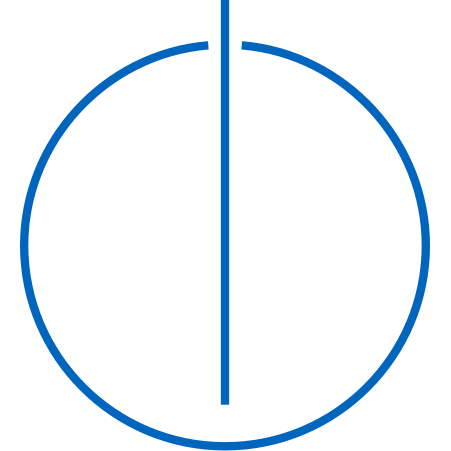
\includegraphics[width=0.15\textwidth]{Informatik_Fakultaet_Logo.png}
\end{titlepage}

\begin{titlepage}
%Dies ist die erste Seite
\centering

\includegraphics[width=0.5\textwidth]{TUM_Logo.png}\par
{\scshape\LARGE Fakultät für Informatik\par}
{\scshape\Large der Technischen Universität München\par}
\vfill
{\large Bachelorarbeit in Informatik: Games Engineering\par}
\vfill
{\LARGE\bfseries Visualisierung von vernetztem Wissen als Graph im virtuellen Raum\par\vspace{0.5cm}}
{\LARGE\bfseries Visualization of interconnected knowledge as a graph in virtual space\par}
\vfill
\begin{tabular}{l l}
	Bearbeiterin:		& Sonja Stefani \\
	Aufgabensteller:	& Prof. Dr. Helmut Krcmar \\
	Betreuer:			& Dimitri Vorona, Dr. Matthias Baume \\
	Abgabedatum:		& 16.04.2018
\end{tabular}\par
\vfill
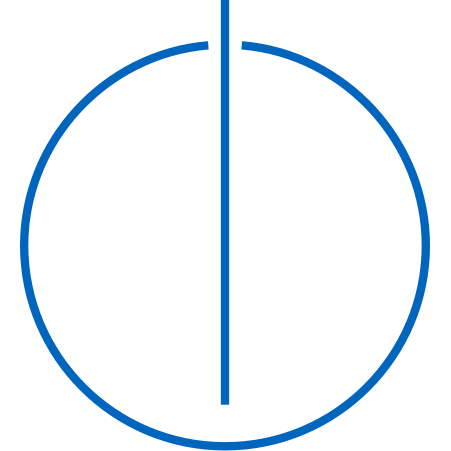
\includegraphics[width=0.15\textwidth]{Informatik_Fakultaet_Logo.png}
\end{titlepage}
\begin{titlepage}
%Dies ist die Erklärung zur handschriftlichen Verfassung
\begin{flushleft}
{\large Ich versichere, dass ich diese Bachelorarbeit selbstständig verfasst und nur die angegebenen Quellen und Hilfsmittel verwendet habe.\par\vspace{2cm}}
% _datum_ & _unterschrift_ (handschriftlich)
\begin{tabular}{l l}
\underline{\hspace{4cm}} & \underline{\hspace{4cm}}
\end{tabular}
\end{flushleft}

\end{titlepage}
\selectlanguage{ngerman}
\begin{abstract}
\addcontentsline{toc}{section}{\protect\numberline{I}{Zusammenfassung/Abstract}}
In dieser Arbeit wird ein Konzept vorgestellt, welches zur Visualisierung von Wissensnetzwerken als Graph im virtuellen Raum verwendet werden kann. Dieses soll Nutzern ermöglichen, sich Wissen nach einem konstruktivistischen Prinzip selber anzueignen. Die Konzipierung erfolgt nach Recherche und Behandlung von Hintergrundwissen zu Graphentheorie, virtueller Realität und der Visualisierung von Informationen. Es beinhaltet das Modellieren von Artikeln eines Wissensnetzwerkes und Verlinkungen dieser als Knoten und Kanten eines gerichteten Graphen. Zur Visualisierung des Graphen wird hierfür ein Algorithmus diskutiert, der Knotenpositionen berechnet, indem anziehende und abstoßende Kräfte zwischen Knoten simuliert werden. Die Darstellung von Informationen erfolgt schließlich in mehreren Schritten, erst über Visualisierung des Graphen des Wissensnetzwerks, dann durch Darstellung eines ausgewählten Artikels und als letztes durch Darstellung der internen Struktur eines Artikels. Einzelne Hürden beim Implementieren des Konzeptes, wie das Verarbeiten von JSON-Nachrichten vom Server des Wissensnetzwerkes und der Verzögerungen im Programmablauf durch Kommunikation mit dem Internet werden besprochen und Lösungen präsentiert.  Das vorgestellte Konzept ermöglicht es Nutzern schließlich, sich eine virtuelle Lernumgebung zu schaffen, in der sich die Relationen zwischen Informationen leichter veranschaulichen lassen.
\end{abstract}
\textbf{\textit{Schlüsselwörter---}} Graphvisualisierung, Virtuelle Realität, Konstruktivismus, Edutainment, Wissensnetzwerke
\newpage
\selectlanguage{english}
\begin{abstract}
In this paper a concept is proposed that can be used to visualize knowledge networks as a graph in virtual space. This shall allow users to acquire knowledge following a constructivist approach. The conceptualization is made after research and discussion of background knowledge for graph theory, virtual reality and the visualization of information. It includes the modelling of articles and their linking in a knowledge network as nodes and edges in a directed graph. An algorithm to visualize the graph and compute node positions by simulating attractive and repulsive forces between nodes is discussed. The visualization of knowledge is then made in multiple steps, first by visualizing the graph of the knowledge network, then by displaying a chosen article and lastly by depicting the internal structure of an article. Single obstacles while implementing the concept are being discussend, like handling JSON messages from the server of the knowledge network and lag in the execution of the program due to communication with the internet. For these obstacles, solutions are introduced. Finally, the presented concept allows users to create virtual learning environments, in which relations between information is depicted in a simpler manner.
\end{abstract}
\textbf{\textit{Keywords---}} graph visualization, virtual reality, constructivism, edutainment, knowledge networks
\selectlanguage{ngerman}
\newpage
\tableofcontents
\newpage
%Ganz ehrlich, Latex ist manchmal Magie
%ich habe eine lokale Datei mit dem gleichen Inhalt wie diese main.tex
%und sie erstellt ein anderes PDF und ich hab nicht den Nerv
%herauszufinden wieso...
%also: hardcoding!
\renewcommand\listfigurename{II Abbildungsverzeichnis}
\listoffigures
\newpage
\addcontentsline{toc}{section}{\protect\numberline{III}{Abkürzungsverzeichnis}}
\section*{III Abkürzungsverzeichnis}
\begin{tabular}{l l}
\textbf{VR} & Virtuelle Realität\\
\textbf{HMD} & head-mounted-display\\
\textbf{$V$} & Menge der Knoten eines Graphen\\
\textbf{$E$} & Menge der Kanten eines Graphen\\
\end{tabular}
\newpage


% Tabellenverzeichnis (noch?) unnötig, da ich keine Tabellen habe
%\listoftables
%\newpage

% Übernehmen der generellen Idee des Proposals
% Motivation und Relevanz

% ANMERKUNG:
% 1. Es wurden noch nicht alle Vorschläge in das Dokument übernommen
% 2. Es fehlen noch Zusammenfassung, Schluss, Gegenüberstellung von Konfigurationen und ein Teil im Konzeptabschnitt
% Der Zitierstil ist, wie verlangt, APA
% Einige der BibTeX-Einträge scheinen nicht richtig dargestellt zu werden, die Verweise im Text sind aber alle korrekt
% an zwei Stellen müssen indirekte Zitate in "Information Visualization" nachgeschaut und die Seitenzahl herausgesucht werden
\section{Einleitung}
\subsection{Motivation}

Lernen und die Kunst des Lernens und Lehrens war schon lange, bevor der erste Computer entwickelt wurde, ein zentraler Teil unserer Menschheit. Auch vor hunderten Jahren gab es bereits Einrichtungen, um den Forschungsdrang und das Bedürfnis der Weiterbildung zu befriedigen \cite[S.~74]{raithel2008einfuhrung}. Mit der Zeit und dem Fortschritt hat der Mensch dieses Wissen auf immer modernere Weise gelernt festzuhalten und zu verbreiten.\\

Während vor den Zeiten der digitalen Speicherung von Informationen noch analoge Medien wie Bücher, Zeitungen oder gar Schallplatten und später Kassetten zum Aneignen von Wissen genutzt wurden, sind heutige Mittel viel zugänglicher und leichter zu verbreiten geworden. In Zeiten des Internets ist man nie weiter als ein paar Mausklicks vom nächsten Artikel entfernt, egal ob man ein neues Instrument lernen will, Tipps zum Kochen sucht oder verstehen will, wie man mit Integralen rechnet. Auch Bildungseinrichtungen sind in Sachen Wissensbereitstellung weitergezogen und verwenden unter anderem Lernplattformen, die online zugänglich sind und es ermöglichen, Vorlesungsmaterialien auszutauschen. Die Plattform Moodle beispielsweise zeigt diese Veränderung ganz deutlich. Sie wurde mit einem konstruktivistischen Lernansatz entwickelt und bringt Lehrende und Lernende online zusammen \cite{Moodle:01}. Inzwischen gibt es über 90.000 Installationen von Moodle in über 200 Ländern \cite{Moodle:02}, darunter auch Einrichtungen wie die Technische Universität München, die Technische Hochschule Ingolstadt oder die Hochschule Augsburg \cite{moodleAugsburg:01}, \cite{moodleTUM:01}, \cite{moodleIngolstadt:01}, um nur einen Bruchteil der teilnehmenden Bildungseinrichtungen zu nennen.\\

Auch Online-Enzyklopädien wie die Encyclopedia Britannica oder Wikipedia stellen Nutzern in wenigen Klicks alles Mögliche an Wissen bereit. Dabei ist das Spektrum breit gefächert: Naturwissenschaften oder Gesellschaftswissenschaften, von Quantenphysik bis zum zweiten Weltkrieg lässt sich alles nachschlagen. Wikipedia bildet dabei zusätzlich eine Besonderheit, da die Enzyklopädie von jedem editiert werden kann. Es ist also nicht nur eine Quelle von Wissen, die immer von allen zugänglich ist, es ist zudem ein kollaboratives Projekt, bei dem Lernende ihr Wissen beisteuern können \cite{Wiki:01}\cite[S.~1]{okoli2009brief}.\\

Die Arten, Wissen zu teilen und etwas zu lernen, sind mit Hilfe des Internets und der Technik also vielfältig geworden. Aber nicht nur die Möglichkeiten, Informationen festzuhalten und zu verbreiten, haben sich verändert. Auch das Konzept des Lernens selber hat sich im Laufe der Zeit verändert. Während früher Lernen als Prozess aufgefasst wurde, der von externen Begebenheiten beeinflusst wurde, wird der Lernprozess heute aufgefasst als "`beeinflusst von interner Strukturiertheit"', wobei der Lernende als aktiver Teilnehmer betrachtet wird \cite[S.~31]{terhart2003constructivism}. Aus einer moderneren Anschauung der Didaktik geht das Konzept des Konstruktivismus hervor. Das passive Dasitzen und Zuhören wird abgelehnt, stattdessen wird der Lernende zunehmend aktiv. Die Lernumgebung rückt in den Vordergrund, soll stimulieren und unabhängiges Lernen anregen. Wissen wird vom Lernenden konstruiert, nicht von außen diktiert \cite[S.~32]{terhart2003constructivism}. Diese Bewegung geht in Richtung einer moderneren Auffassung des Lernens, ein Lernen, bei dem der Lernwillige sich das Wissen selbst erschließt und aneignet.\\

Mithilfe von virtueller Realität (VR), einer Technik, um Nutzern Immersion in einer virtuelle Umgebung zu ermöglichen, soll in dieser Arbeit nun ein Konzept vorgestellt werden. Mit diesem sollen sich Nutzer frei in einem Ausschnitt der Wikipedia bewegen können, also von Artikel zu Artikel. Sie sollen sich, in Anlehnung an den Konstruktivismus, selber einen Überblick über die Verbindungen zwischen Artikeln schaffen können und in einer isolierten Umgebung Wissen aus besagten Artikeln aneignen können.\\

Um diesen Vorschlag umzusetzen, ist es nötig, sich mit verschiedenen Fragen auseinanderzusetzen und geeignete Lösungen zu finden. In dieser Arbeit soll unter anderem erläutert werden, wie Wissensnetzwerke, wie die Wikipedia, aufgebaut sind und welche Eigenschaften die Struktur eines Wissensnetzwerks ausmachen. Auch soll erläutert werden, wie die Menge an Wissen einem Nutzer übersichtlich dargestellt werden kann. Zudem wird darauf eingegangen, wie die einzelnen Artikel und darin enthaltene Informationen im virtuellen Raum dargestellt werden können. Mit dem gesammelten Wissen soll schließlich erläutert werden, wie ein Prototyp zur Visualisierung von vernetztem Wissen im virtuellen Raum implementiert werden kann.\\

\subsection{Hintergrund und ähnliche Werke}
Mit der Idee des Konstruktivismus adäquate Lernumgebungen zu schaffen, wurde beispielsweise bereits im Bereich des Edutainments erfolgreich bewerkstelligt \cite{bertacchini2012motivating}. Zahlreiche Programme zur spielerischen Aneignung von Konzepten und Wissen sind bereits auf dem Markt und stellen eine Lernumgebung bereit, die den Lernprozess anregt und den Nutzer aktiv werden lässt.\\

Es gibt mehrere Studien zur Effektivität und zum Nutzen von VR in Verbindung mit Lernsituationen. In \citeA{strickland1996virtual} wird eine Studie vorgestellt, bei der zwei autistische Kinder in einer Szene in der virtuellen Umgebung ein bekanntes Objekt erkennen und zu diesem gehen sollen. Die verwendete Szene ist eine Straße mit einem Stoppschild und einem Auto als zu erkennendes Objekt. Die Studie kommt zu dem Ergebnis, dass die Kinder die Technik akzeptieren, die virtuelle Welt von der echten unterscheiden können und auch auf diese reagieren können. In einer anderen Studie aus \citeA{park2011virtual} wurden 91 Schizophrenie-Patienten in zwei Gruppen aufgeteilt. Beide sollten an "`social skill training"' teilnehmen, welches zur sozialen Rehabilitation eingesetzt wird. Hierbei wurde eine Gruppe mithilfe von VR trainiert, die andere nicht. Die Studie kam zu dem Ergebnis, dass die Gruppe, die VR verwendete, mehr Interesse am Training zeigten und motivierter teilnahmen.\\

In \citeA{kaufmann2000construct3d} wird eine Anwendung vorgestellt, die in der Bildung verwendet werden soll. Nutzer können mithilfe dieser Anwendung dreidimensionale Objekte in einem virtuellen Raum platzieren und haben zudem die Möglichkeit, sich in diesem frei zu bewegen. Eine kurze Evaluation mit 14 Teilnehmern ergibt, dass das Konzept und deren Umsetzung in VR sehr gut aufgenommen wurde. Ein weiteres System zur Einbettung von Anwendungen in virtueller Realität stammt von \citeA{carlsson1993dive}. Das hier vorgestellte System, DIVE, ermöglicht Kollaboration mit mehreren Nutzern, die in der virtuellen Umgebung von sichtbaren Objekten dargestellt werden. Das System kann als Grundlage verwendet werden, um verschiedene Anwendung so umzusetzen, dass sie in VR mit anderen Nutzern zusammen benutzt werden können.\\

Eine weitere Arbeit, die einen ähnlichen Gedanken verfolgt, wie das hier vorgestellte Konzept, kommt von \citeA{munzner1995visualizing}. Sie stellen in ihrem Werk eine Anwendung vor, welche die Struktur von Teilen des Internets und deren Vernetzung in dreidimensionalem, hyperbolischen Raum darstellen soll.\\

\section{Hintergrundwissen}

\subsection{Anwendungen im virtuellen Raum}

Das Konzept der Immersion in einer virtuellen Welt existiert bereits seit über 50 Jahren. Einen Überblick bieten \citeauthor{mazuryk1996virtual}: Bereits in den Jahren 1960 bis 1965 wurden umfassende multisensorischen Systeme formuliert \cite[S.~2]{mazuryk1996virtual}. Etwas später wurde das erste "`Head Mounted Display"' (HMD) von Sutherland gebaut, welches bereits Tracking der Kopfposition unterstützt hat \cite{sutherland1968head}. Das HMD verwendet zwei Linsen, die für die beiden Augen des Menschen versetzte Bilder anzeigen, um einen räumlichen Effekt zu bewirken. Sutherlands Konzept hat damals allerdings noch vorgesehen, die Position und Rotation des HMD mit einem Verbindungsarm zu messen, siehe Abb.~\ref{sutherlandHMD}.\\

\begin{figure}[h!]
\centering
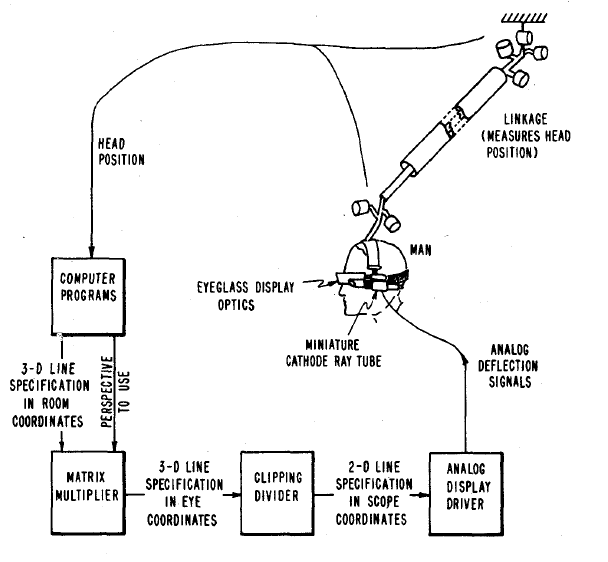
\includegraphics[width=0.95\textwidth]{Isdale_HMD_concept.png}
\caption[Konzept zur Realisierung eines VR-Systems]{Konzept zur Realisierung eines VR-Systems, Quelle:\protect\cite{sutherland1968head}}
\label{sutherlandHMD}
\end{figure}

Modernere Systeme verwenden stattdessen Kameras oder Sensoren, um dem Nutzer die Möglichkeit zu bieten, sich uneingeschränkt im virtuellen Raum zu bewegen \cite{vive:01}.
Nach Sutherland folgten weitere Systeme, die die Simulation einer virtuellen Realität als Ziel hatten. Ein Beispiel davon ist ein Flugsimulator, welcher 1982 an den US Air Force's Medical Research Laboratories von Thomas Furness entwickelt wurde \cite[S.~2]{mazuryk1996virtual}. Seit 1985 sind auch die ersten VR-Systeme kommerziell verfügbar.\\

Eine klare Definition für die Begriffe "`virtueller Raum"', "`virtuelle Realität"' oder auch "`virtuelle Umgebung"' ist schwer zu formulieren. Alle drei Begriffe werden in dieser Arbeit und auch in der meisten Literatur zu dem Thema synonym verwendet \cite[S.~3ff]{mazuryk1996virtual}, \cite[S.~4]{brooks1992research}. Diese Begriffe  werden in der Literatur unterschiedlich definiert.\\

Nach \citeA[S.~2]{brooks1992research} ist bei dem Begriff "`virtuelle Umgebung"' eine dreidimensionale Echtzeitdarstellung einer modellierten Welt gemeint, bei der der Benutzer die Welt durch passende Anzeigetechnologie betrachten kann und direkt mit ihr interagieren kann. Isdale erwähnt, dass der Begriff "`virtuelle Realität"' sich für manche Menschen auf spezielle Technologien, wie dem HMD, beschränkt und für andere wiederum auch Filme oder gar die eigene Vorstellungskraft umfasst \cite{isdale1998virtual}. \citeA[S.~23]{franchi1994virtual} beschreibt virtuelle Realität als computer-generierte sensorische Erfahrung, die den Teilnehmer so in eine Welt eintauchen lässt, dass er die virtuelle Welt und die reale Welt kaum mehr unterscheiden kann. Hierbei sollen Computergraphik, Ton und Bilder verwendet werden, um eine elektronische Version echter Szenarien nachzubilden. \citeA[S.~127]{zeltzer1992autonomy} schreibt, dass für virtuelle Umgebungen drei Aspekte umgesetzt werden müssen, Autonomie des Systems, Interaktion mit dem System und Präsenz in dem System. In einem Würfel mit den drei genannten Aspekten als Achsen eines zugrunde liegenden Koordinatensystems stellt er dessen Zusammenhang dar, siehe Abb.~\ref{zeltzerCube}. Virtuelle Realität liegt in diesem Würfel an der Ecke, an der alle drei Aspekte ihren höchsten Wert erreichen \cite[S.~129]{zeltzer1992autonomy}.\\

\begin{figure}[h!]
\centering
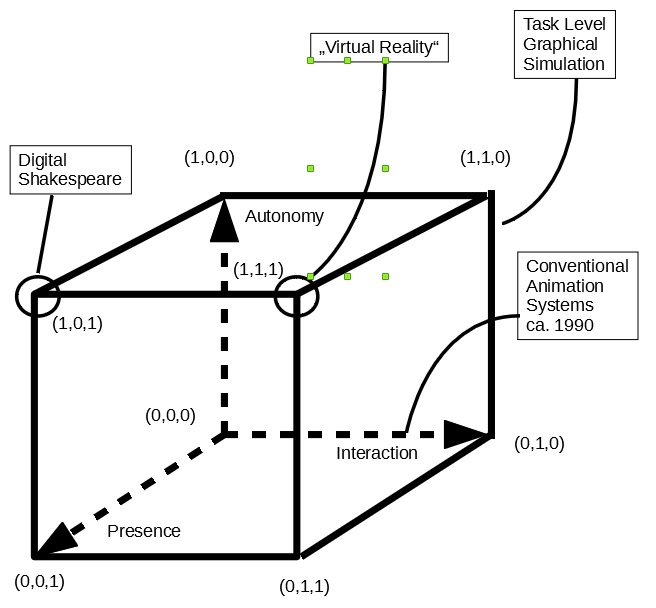
\includegraphics[width=0.95\textwidth]{zeltzersCube.png}
\caption[Würfel zur Darstellung des Zusammenhangs zwischen Autonomie, Interaktivität und Präsenz]{Würfel zur Darstellung des Zusammenhangs zwischen Autonomie, Interaktivität und Präsenz, adaptiert aus~\protect\citeA{zeltzer1992autonomy}}
\label{zeltzerCube}
\end{figure}

Die ersten Anwendungen, die virtuelle Realität und Präsenz in einer virtuellen Welt genutzt haben, wurden von Forschungsinstituten und der Industrie entwickelt, wie Flugsimulatoren, Anwendungen zur Visualisierung von Daten und Anwendungen zur Betrachtung von architektonischen Modellen \cite[S.~6]{mazuryk1996virtual}.\\

\newpage
\subsection{Grundlagen der Graphentheorie}
Um das in dieser Arbeit vorgestellte Konzept zur Visualisierung der Wikipedia als dreidimensionalen Graphen umsetzen zu können, ist es zuerst nötig, zu verstehen, was ein Graph ist.  Die folgenden Erklärungen und Definitionen sind aus \citeA{diestel2017graph} und \citeA{arumugam2016handbook} entnommen. Es werden hier nicht alle Aspekte der Graphentheorie erwähnt, speziell werden nur endliche Graphen behandelt.\\

In der Mathematik bezeichnen wir $G$ als Graph, bestehend aus einem Tupel $(V, E)$, also $G=(V,E)$. Die Menge $V$ bezeichnet die Menge aller Knoten (oder Vertices) des Graphen $G$, die Menge $E$ bezeichnet alle Kanten des Graphen $G$. Für die Menge $E$ gilt in einem ungerichteten Graphen $E \subseteq [V]^2$, sie ist also eine Menge von Teilmengen, die immer aus zwei Elementen besteht und deren Elemente aus $V$ stammen. Hier ist es wichtig, zu beachten, dass die geschriebene Reihenfolge von Elementen einer Menge bei einem ungerichteten Graphen irrelevant ist und $\{x, y\} = \{y, x\}$ gilt. Eine Kante $e \in E$ hat die Form $e = \{x, y\}$ mit $x,y \in V$. Ein Graph $G$ kann dargestellt werden, in dem alle Elemente aus $V$ als Punkte dargestellt werden, und alle Elemente aus $E$ als Linien zwischen diesen Punkten. Dabei geben die beiden Einträge in einem $e \in E$ an, zwischen welchen beiden Punkten eine Linie gezeichnet wird. Abb. \ref{example_graph_brandstaedtetal} zeigt die Darstellung des Graphen $G = (V, E)$ mit $V = \{a, b, c, d\}$ und $E = \{\{a, b\}\{a, c\}\{a, d\}\}$.\\

\begin{figure}[h!]
\centering
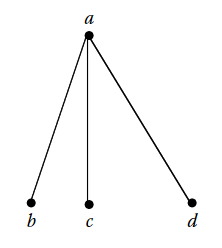
\includegraphics[width=0.5\textwidth]{example_graph_BrandstaedtEtAl.png}
\caption[Beispiel eines ungerichteten Graphen]{Beispiel eines ungerichteten Graphen, Quelle: \protect\citeA{arumugam2016handbook}}
\label{example_graph_brandstaedtetal}
\end{figure}

Wir nennen zwei Knoten $v, w \in V$ Nachbarn oder auch adjazent, falls es eine Kante $e \in E$ gibt, für die gilt $e=\{v, w\}$. In Abb.~\ref{example_graph_brandstaedtetal} sind demnach beispielsweise a und b Nachbarn. Zwei Kanten $e, f \in E$ mit $e \neq f$ sind adjazent, falls beide an dem gleichen Knoten hängen, also $e = \{x, y\}$ und $f=\{x, z\}$. Der Grad eines Knoten $deg(v)$ mit $v \in V$ ist die Anzahl an Kanten, in denen $v$ vorkommt. In Abb.~\ref{example_graph_brandstaedtetal} gilt $deg(a)=3$, $deg(b) = deg(c) = deg(d) = 1$.\\

Sei $G = (V, E)$. Wir bezeichnen $G_{sub} = (V_{sub}, E_{sub})$, wenn gilt $V_{sub} \subseteq V$ und $E_{sub} \subseteq E$. Wir sagen auch, dass $G$ den Graphen $G_{sub}$ enthält \cite[S.~5]{arumugam2016handbook}.\\

Ein Weg bezeichnet einen Graphen $W = (V, E)$ mit $V = \{x_0, x_1, \dots, x_k\}$ und $E = \{\{x_0, x_1\}, \{x_1, x_2\}, \dots, \{x_{k-1}, x_k\}\}$, wobei alle $x_i$ unterschiedliche Knoten sind. Intuitiv ist ein Weg in einem Graphen eine Reihe von aneinanderhängenden Knoten, wie in Abb.~\ref{example_graph_way_diestel} aus \citeA{diestel2017graph} zu sehen. Wir schreiben einen Weg mit $E = \{\{x_0, x_1\}, \{x_1, x_2\}, \dots,$ $\{x_{k-1}, x_k\}\}$ auch abgekürzt als $W = x_0\dots x_k$ und sagen, der Weg führt von $x_0$ nach $x_k$.\\

Was in Abb.~\ref{example_graph_way_diestel} auch zu sehen ist, sind Kreise oder auch Zyklen. Betrachten wir einen Weg $W = x_0\dots x_{k-1}$ mit $k \geq 3$. Fügen wir zu diesem Weg eine Kante $\{x_{k-1}, x_0\}$ hinzu, so bezeichnen wir den Graph $W_{neu}$, den wir erhalten, als Kreis oder Zyklus. In Abb.~\ref{example_graph_cycle_diestel} aus \citeA{diestel2017graph} ist ein solcher Kreis innerhalb eines Graphen dargestellt.\\

\begin{figure}[h!]
\centering
\begin{subfigure}[t]{0.45\textwidth}
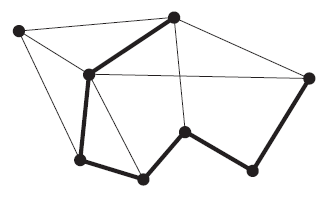
\includegraphics[height=2.5cm]{example_graph_way_diestel.png}
\caption[Beispiel eines Weges innerhalb eines Graphen]{Beispiel eines Weges innerhalb eines Graphen, Quelle: Adaptiert aus \protect\citeA{diestel2017graph}}
\label{example_graph_way_diestel}
\end{subfigure}
\begin{subfigure}[t]{0.45\textwidth}
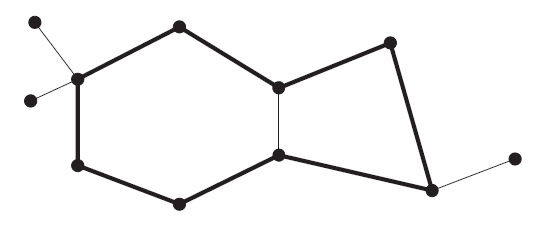
\includegraphics[height=2.5cm]{example_graph_cycle_diestel.png}
\caption[Beispiel eines Kreises innerhalb eines Graphen]{Beispiel eines Kreises innerhalb eines Graphen, Quelle: Adaptiert aus \protect\citeA{diestel2017graph}}
\label{example_graph_cycle_diestel}
\end{subfigure}
\caption{Zwei Graphen mit je einem Weg oder Kreis eingezeichnet}
\end{figure}

Ein planarer Graph ist ein Graph, der so gezeichnet werden kann, dass keine zwei Kanten sich in einem anderen Punkt treffen, als in einem Endvertex. Ein solcher Graph hat also keine sich kreuzenden Kanten. Die Zeichnung eines planaren Graphs nennt man auch eben.\\

Für das vorgestellte Konzept ist es außerdem wichtig, zu verstehen, was ein gerichteter Graph oder auch Digraph ist. Das hier vorgestellte Wissen stammt hauptsächlich aus \citeA{bang2008digraphs} und zum Teil aus \citeA{arumugam2016handbook}. Ein solcher Graph $G$ besteht immer noch aus zwei Mengen $(V, E)$, wobei die Menge $E$ nicht mehr nur eine Menge von Teilmengen ist. In \citeA{bang2008digraphs} wird die Menge $E$ als $A$ für "`arcs"' bezeichnet, da wir aber in dieser Arbeit hauptsächlich mit gerichteten Graphen arbeiten, belassen wir die Benennung der Kantenmenge bei $E$. Die Menge der Kanten besteht in einem gerichteten Graphen aus geordneten Paaren von Elementen aus $V$. Ein Eintrag der Kantenmenge hat also die Form $(x, y)$ mit $x,y \in V$. Ein Beispiel aus \citeA{bang2008digraphs} für einen gerichteten Graph ist in Abb.~\ref{example_digraph_BangJensenGutin} zu sehen. Der dargestellte Graph besteht aus einer Knotenmenge $V = \{u, v, w, x, y, z\}$ und einer Kantenmenge $E = \{(x, z), (y, z), (z, u), (u, v), (u, w), (w, u)\}$. Wir sagen, dass eine Kante $(u, v)$ den Knoten $u$ verlässt und auf den Knoten $v$ zeigt. Die Knoten $u$ und $v$ sind, wie bei ungerichteten Graphen, adjazent zueinander.\\

\begin{figure}[h!]
\centering
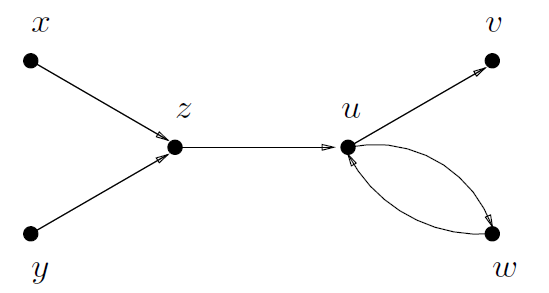
\includegraphics[width=0.5\textwidth]{example_digraph_BangJensenGutin.png}
\caption[Beispiel eines gerichteten Graphen]{Beispiel eines gerichteten Graphen, Quelle: \protect\cite{bang2008digraphs}}
\label{example_digraph_BangJensenGutin}
\end{figure}

Ein Knoten $x \in V$ in einem gerichteten Graphen hat nun eingehende und ausgehende Nachbarn und demzufolge auch einen Eingangs- und Ausgangsgrad. In Abb.~\ref{example_digraph_BangJensenGutin} hat beispielsweise der Knoten $z$ einen Eingangsgrad von $deg^-(u) = 2$ und einen Ausgangsgrad von $deg^+(u) = 2$.\\

Als letztes in diesem Kapitel wird noch die Breitensuche angesprochen \cite[S. 92f]{bang2008digraphs}. Ursprünglich findet dieser Algorithmus von einem Knoten $s$ ausgehend die Distanzen zu allen anderen Knoten des Graphen. Hierbei werden alle von Knoten $s$ erreichbaren Nachbarn durchgangen und in eine Warteschlange eingefügt. Wurden alle Nachbarn ermittelt, geht der Algorithmus zum nächsten Knoten in der Warteschlange über und erkundet alle von hier aus erreichbaren Nachbarn. Zusätzlich werden bei jedem Schritt die Distanz zum aktuell betrachteten Nachbarn aktualisiert. In der Umsetzung des in dieser Arbeit vorgestellten Konzepts wird die Breitensuche abgewandelt. Sie wird hier nicht verwendet, um Distanzen zu ermitteln, sondern um einen unbekannten Graph ausgängig von einem bekannten Knoten zu erkunden und alle unbekannten Knoten und Kanten zu finden. Knoten, die bereits erkundet wurden, werden in der Warteschlange nicht hinzugefügt.\\

\newpage
\subsection{Visualisierung von Informationen}
Die Visualisierung von Daten ist in vielen Teilbereichen der Natur- und Gesellschaftswissenschaften ein gefragtes Thema. \citeA[S.~89]{meyer2000visualization} beispielsweise schreiben: „Visualization can be defined as the use of computer-supported, interactive, and dynamic visual representations of data to amplify cognition. Goals are discovery, decision-making and explanation.“ In \citeA[S.~6]{card1999readings} findet sich der erste Satz dieses Zitats unverändert ebenfalls als Definition von Visualisierung wieder.\\

Sie erwähnen zudem, dass durch die Evolution des Computers grafische Darstellung möglich gemacht wurden, die im Hinblick auf die Vergangenheit verbessert sind und dabei Interaktivität bieten \cite[S.~1]{card1999readings}. Allein das Aufschreiben von Zwischenschritten bei der schriftlichen Multiplikation hilft bereits, das Gedächtnis zu erweitern und die Multiplikation schneller durchzuführen, als ohne Stift und Papier \cite[S.~2]{card1999readings}. Dass zudem wichtige Informationen klar dargestellt werden müssen, damit sie leicht verständlich sind, zeigt der Vergleich von Abb.~\ref{ORing_bad} und Abb.~\ref{ORing_good}. Beide Diagramme sollen veranschaulichen, wie bei einem Raketenstart die Außentemperatur Schaden an der Versiegelung der Verbindungen der einzelnen Raketenteile macht. In Diagramm~\ref{ORing_bad} wurden die Temperaturen seitwärts als Text in den Abbildungen der Rakete eingetragen und so schwer lesbar gemacht. Die verschiedenen Raketen stehen dabei für verschiedene Raketenstarts und dort gemessene Werte. In Abb.~\ref{ORing_good} hingegen wurden alle Raketenstarts als Punkte in einem Graph eingezeichnet, der die Relation zwischen Temperatur und Grad des Schadens darstellt. Während aus Abb.~\ref{ORing_bad} nicht leicht ersichtlich ist, ob die Rakete bei kälteren Temperaturen wirklich Schaden nimmt, stellt Abb.~\ref{ORing_good} klar da, dass es eine Verbindung zwischen kalten Temperaturen und Schaden an einer Rakete gibt. Nach \citeA[S.~373]{freitas2002evaluating} sollen sowohl die visuelle Darstellung als auch die Interaktionstechniken nicht beeinflussen dürfen, wie ein Nutzer für die bereitgestellten Daten weiterverwendet. \citeA[S.~109]{brath1997metrics} schreibt zu dem Thema, dass eine komplexe Visualisierung schwerer zu verstehen ist, als eine simple und dass eine effektive Visualisierung die Komplexität reduzieren sollte.\\

\begin{figure}[h!]
\centering
\begin{subfigure}[b]{0.9\textwidth}
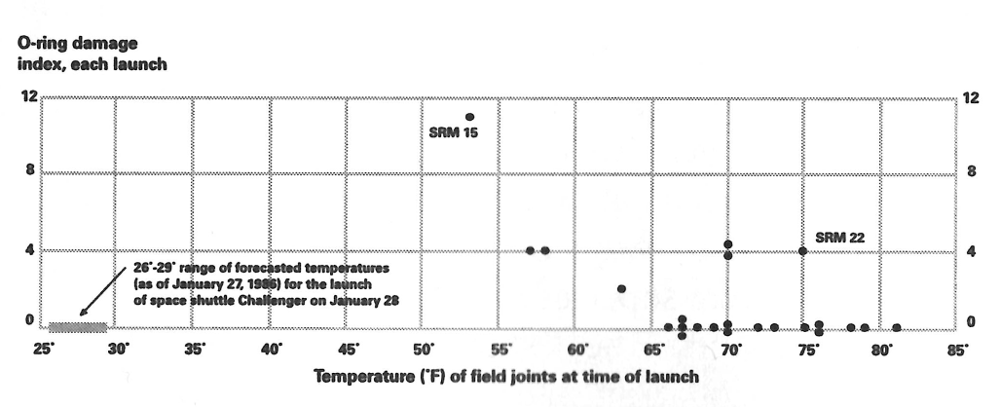
\includegraphics[width=\textwidth]{ORing_good.png}
\caption[Diagramm zur Verdeutlichung der Korrelation zwischen Schaden an einer Rakete und Außentemperatur]{Diagramm zur Verdeutlichung der Korrelation zwischen Schaden an einer Rakete und Außentemperatur, Quelle: \protect\citeA{card1999readings}}
\label{ORing_good}
\end{subfigure}
\begin{subfigure}[b]{0.9\textwidth}
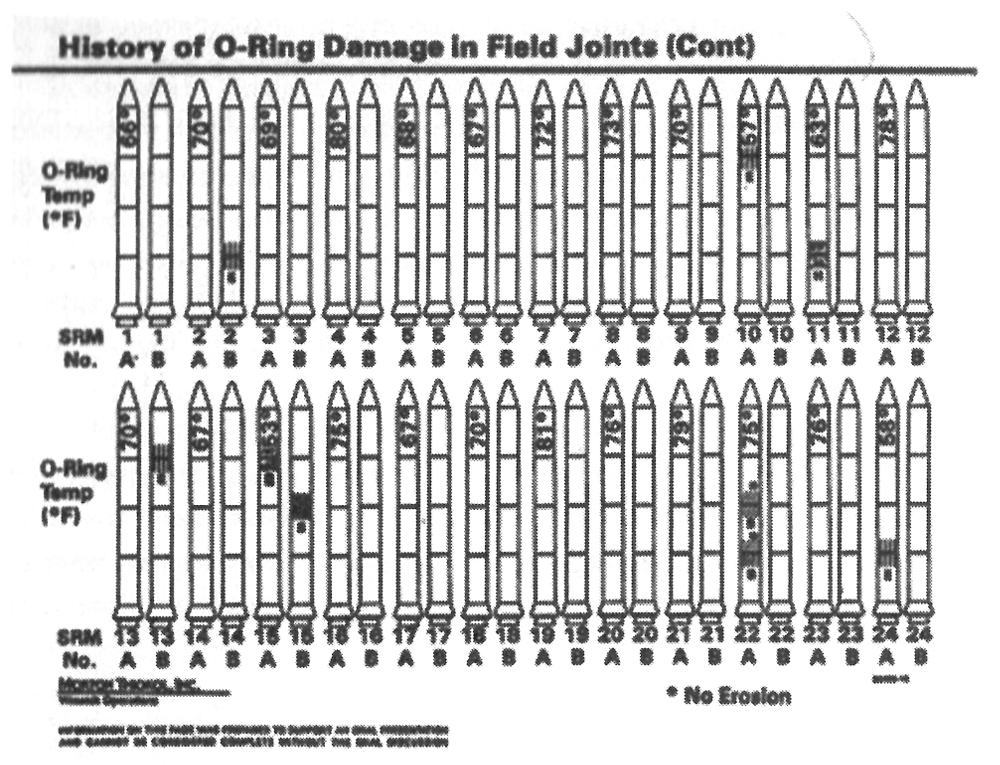
\includegraphics[width=\textwidth]{ORing_bad.png}
\caption[Diagramm, in dem Informationen über Temperatur und Schaden in Abbildungen von Raketen eingezeichnet ist]{Diagramm, in dem Informationen über Temperatur und Schaden in Abbildungen von Raketen eingezeichnet ist, Quelle: \protect\citeA{card1999readings}}
\label{ORing_bad}
\end{subfigure}
\caption{Zwei Diagramme, die beide verdeutlichen sollen, ob Temperaturen bei Raketenstarts wesentlich Schaden an einer Rakete anrichten können}
\end{figure}

Informationen können auf verschiedene Arten für einen Betrachter dargestellt werden. Abb.~\ref{from_data_to_visualization} verdeutlicht den Weg von gegebenen Daten zur grafischen Repräsentation. Der erste Schritt hier ist es, die rohen Daten in Relationen umzuformen. Diese lassen sich dann in einer Tabelle von Daten darstellen, was in Abb.~\ref{from_data_to_visualization} vom Kasten "`Data Tables"' repräsentiert wird. Als nächste ist es möglich, diese Daten in eine visuelle Struktur zu packen. Um eine gute visuelle Struktur zu erhalten, ist es nötig, die Daten bei der Umwandlung zu erhalten \cite[S.~5]{card1999readings}. Die Umwandlung zu einer visuellen Darstellung ist meist auf mehrere Arten und Weisen möglich. Nicht alle möglichen Darstellungen garantieren aber, nicht versehentlich zusätzliche Informationen darzustellen oder überhaupt verständlich zu sein, wie Abb.~\ref{ORing_bad} verdeutlicht. Der letzte Schritt, der in Abb.~\ref{from_data_to_visualization} eingezeichnet ist, ist der Kasten "`Views"'. Man erhält verschiedene Darstellung durch interaktive Manipulation der Visualisierung. Diese Manipulation kann beispielsweise durch Anpassen von Parametern erfolgen oder auch durch Auswählen von erweiterten Ansichten möglich gemacht werden. So kann eine Visualisierung beispielsweise eine Übersicht über die Informationen bieten und der Nutzer erweiterte Informationen ausklappen \cite[S.~31]{card1999readings}. Ein simples Beispiel dafür findet sich in vielen Programmen wieder, die mit einer Systemleiste hinter Einträgen wie "`Datei"', "`Bearbeiten"' oder "`Hilfe"' weitere Auswahlmöglichkeiten verstecken.\\

\begin{figure}[h!]
\centering
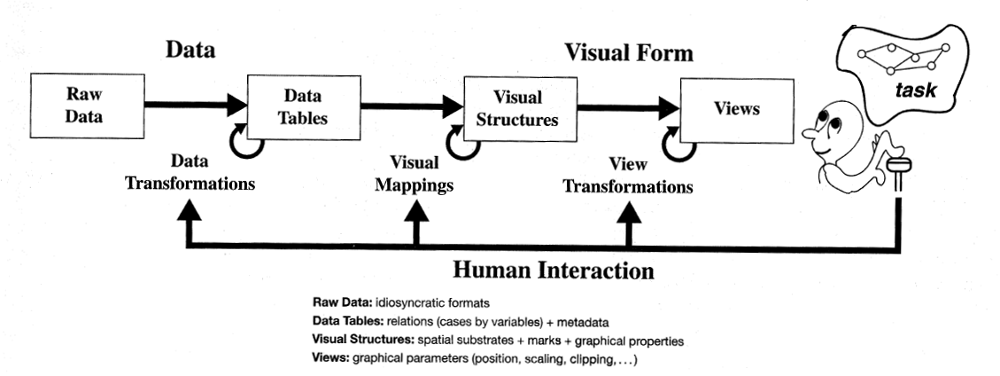
\includegraphics[width=0.9\textwidth]{from_data_to_visualization.png}
\caption[Prozess der Umwandlung von rohen Daten in Visualisierungen]{Prozess der Umwandlung von rohen Daten in Visualisierungen, Quelle: \protect\citeA{card1999readings}}
\label{from_data_to_visualization}
\end{figure}

Informationen können zudem in verschiedenen Dimensionen dargestellt werden. Es gibt sowohl eindimensionale visuelle Strukturen als auch zweidimensionale, dreidimensionale oder mehrdimensionale \cite[S.~57f]{card1999readings}). Eindimensionale Strukturen werden häufig als Teil von zweidimensionalen oder dreidimensionalen Visualisierungen verwendet \cite[S.~58]{card1999readings}. Zweidimensionale Strukturen werden häufig für Diagramme oder geographische Daten verwendet \cite[S.~59]{card1999readings}. Dreidimensionale Strukturen können sowohl echte dreidimensionale Daten darstellen (wie beispielsweise eine Repräsentation des menschlichen Gehirns), oder auch abstraktere Daten auf drei Dimensionen kombinieren (wie beispielsweise eine Darstellung der Nähe zwischen verschiedenen Internetseiten als dreidimensionaler Graph) \cite[S.~60]{card1999readings}.\\

Mit moderner Technologie ist es nun auch möglich, Visualisierungen von Informationen in eine virtuelle Realität einzubetten. Der Vorteil von VR ist, dass ein Nutzer die Information räumlich wahrnehmen kann und ein Gefühl von Tiefe hat \cite[S.~64]{bryson1996virtual}. Sie bietet die Möglichkeit, intuitiv und in Echtzeit Informationen zu erkunden. Probleme bei der Visualisierung in virtueller Realität sind hingegen hohe Berechnungskosten \cite[S.~65]{bryson1996virtual}. Auch gibt es Leute, denen bei der Betrachtung einer virtuellen Umgebung durch ein HMD oder beim Absetzen des HMD schwindelig wird \cite[S.~271]{kaufmann2000construct3d}.\\

\newpage
\subsection{Algorithmen zur Visualisierung von Graphen}
Um einen Graphen zu zeichnen, gibt es, je nach Eigenschaften des Graphen, verschiedene Algorithmen. Diese sollen im Folgenden vorgestellt und verglichen werden. Nicht erwähnt werden Algorithmen, die speziell konzipiert wurden, um gewissen Eigenschaften wie Hierarchie darzustellen. Die hier vorgestellten Algorithmen wurden konzipiert, um einen visuell ästhetischen, ungerichteten Graphen zweidimensional darzustellen. Sie werden hier vorgestellt, da sie leicht verständlich und leicht anpassbar sind.\\

Prinzipiell können Algorithmen zur Visualisierung eines beliebigen, ungerichteten Graphen auf verschiedenen Konzepten basieren. Die hier vorgestellten Algorithmen basieren entweder auf dem Prinzip des "`force-directed placement"' \cite{eades1984heuristic} \cite{kamada1989algorithm} \cite{fruchterman1991graph} oder auf dem Prinzip des "`simulated annealing"' \cite{davidson1996drawing}.\\

Die auf "`force-directed placement"' basierenden Algorithmen betrachten den Graph als eine Kombination aus Ringen und Federn, ursprünglich vorgeschlagen von Eades 1984 \cite[S.~149]{eades1984heuristic}. Die Knoten des Graphen bilden hier Ringe, die Kanten des Graphen werden als Federn modelliert, die diese Ringe verbinden. Die auf "`simulated annealing"' basierenden Algorithmen hingegen schlagen pro Iterationsschritt ein neues Layout für den Graphen vor und behalten oder verwerfen dieses nach Evaluation mit einer Kostenfunktion \cite[S.~303ff]{davidson1996drawing}.\\

In \citeA[S.~149f]{eades1984heuristic} werden die Knoten des Graphen, der gezeichnet werden soll, zufällig im Raum platziert. Als nächstes wird ein Algorithmus auf den Graphen angewandt, der die Positionen der Knoten anpasst und versucht, eine möglichst gleichmäßige Verteilung zu erzielen. Der ursprüngliche Algorithmus ist in Abb.~\ref{eades_algorithm} zu sehen.\\

\begin{algorithm}
\caption{Kräfte basierender Algorithmus zur Graphvisualisierung, Quelle: \protect\citeA{eades1984heuristic}}
\label{eades_algorithm}
\begin{algorithmic}
	\State \text{algorithm SPRING(G:graph);}
	\State \text{place vertices of G in random locations;}
	\State \text{repeat M times}
		\State \hspace{\algorithmicindent} \text{calculate the force on each vertex;}
		\State \hspace{\algorithmicindent} \text{move the vertex C4*(force on vertex)}
	\State \text{draw graph on CRT or plotter.}
\end{algorithmic}
\end{algorithm}

In Algorithmus~\ref{eades_algorithm} ist $G$ der Graph, der gezeichnet werden soll. Die Zahl $M$ gibt an, wie häufig die Platzierung der Knoten verfeinert wird. Laut Eades 1984 erreichen nach 100 Simulationsschritten, also $M=100$, fast alle Graphen einen Status von minimaler Energie. Der Wert $C4$ ist eine Konstante, die experimentell ermittelt wird, um ein gutes Layout zu produzieren.\\

Die Kraft, die auf einem Ring oder Vertex wirkt und so dessen Position verändert, ermittelt sich in zwei Schritten. Sie ist absichtlich nicht realistisch gestaltet, da für ein visuell ansprechendes Ergebnis keine realistische Simulation nötig ist. Als erstes werden die Kräfte berücksichtigt, die die Federn, die am Ring hängen, auf diesen ausüben. Für diese Berechnung werden die Distanzen der Nachbarn des Ringes oder Vertex ermittelt. Die Formel zur Berechnung der Kraft, die ein adjazenter Knoten auf einen Ring ausübt, ist
\begin{equation} \label{eades_attractiveForces}
C1*log(\enskip\frac{d}{C2}\enskip).
\end{equation}
In dieser Formel sind $C1$ und $C2$ wieder Konstanten, die ermittelt werden müssen. Der Wert $d$ ist die Distanz zum Knoten, der die Kraft auf den Ring ausübt.\\

Als nächstes werden die abstoßenden Kräfte berechnet, die von nicht-adjazenten Knoten aus auf den betrachteten Ring wirken. Hierfür verwendet Eades die Formel
\begin{equation} \label{eades_repulsiveForces}
\frac{C3}{\sqrt(d)}.
\end{equation}
Auch hier ist $C3$ ein Wert, der ermittelt werden muss und $d$ wieder die Distanz zwischen den betrachteten Knoten.\\

Ein weiterer Vorschlag zur Visualisierung eines Graphen, basierend auf dem bereits vorgestellten Feder-und-Ring-Prinzip, kommt von Kamada und Kawai. Das dort vorgestellte Prinzip versucht allerdings keine akzeptablen Formeln zur annähernden Berechnung von Kräften zu präsentieren, sondern die totale Energie des Systems zu minimieren und durch diese Minimierung geeignete Positionen für die Knoten des Graphen zu finden. Die Formel zur Berechnung der Energie des Systems aus Ringen und Federn ist hierbei
\begin{equation} \label{kamadaKawaiEnergy}
E=\sum_{i=1}^{n-1} \sum_{j=i+1}^{n} \enskip \frac{1}{2} \enskip k_{ij} \enskip (|p_i \enskip – \enskip p_j| \enskip - \enskip l_{ij})^2.
\end{equation}
In dieser Formel repräsentiert $p$ einen Knoten aus $V$ als Partikel in einer Ebene. $n$ ist die Anzahl an Knoten, also $n=|V|$. Der Wert $l_{ij}$ gibt die anfangs gewünschte Länge zwischen zwei Knoten $v_i$ und $v_j$ an. Der Wert $k_{ij}$ gibt die Stärke der Feder zwischen $v_i$ und $v_j$ an. Im nächsten Schritt versuchen Kamada und Kawai, die Energie $E$ für die Positionen der Partikel $p_0 \dots p_n$ zu minimieren, die zur Berechnung der Klammer in~\ref{kamadaKawaiEnergy} verwendet werden. Sie berechnen mit Hilfe der Newton-Raphson Methode ein lokales Minimum von $E$ \cite[S.~9]{kamada1989algorithm}.\\

Der dritte und letzte hier vorgestellte Algorithmus, der auf der Berechnung von Kräften basiert und den Graph als Sammlung von Ringen und Federn betrachtet, kommt von \citeA{fruchterman1991graph}. Sie nennen zwei Prinzipien, nach denen ein Graph gezeichnet werden soll:
\begin{quote}
\begin{enumerate}
\item Vertices, die per Kante verbunden sind, sollen nah aneinander gezeichnet werden.
\item Vertices sollen nicht \textit{zu} eng aneinander gezeichnet werden.
\end{enumerate}
\end{quote}
Zusätzlich stützen sie sich auf die Vorgehensweise von Eades, die Berechnungen der Kräfte unrealistisch zu gestalten und anziehende Kräfte nur zwischen benachbarten Knoten zu berechnen.  Ihr vorgeschlagener Algorithmus zur Visualisierung eines Graphen besteht aus drei Schritten:
\begin{enumerate}
\item Berechne zuerst die anziehenden Kräfte, die auf einen Knoten wirken,
\item berechne dann die abstoßenden Kräfte, die auf einen Knoten wirken,
\item begrenze die Verschiebung schließlich auf eine gegebene Temperatur.
\end{enumerate}
Die hier genannte Temperatur bezieht sich auf den Rückgabewert einer Funktion, die pro Iterationsschritt des Algorithmus die Temperatur verringert. Sie wird dann verwendet, um die Verschiebung von Knoten immer geringer werden zulassen und den Graphen damit "`abzukühlen"' \cite[S.~1132f]{fruchterman1991graph}. Die Formeln zur Berechnung der anziehenden und abstoßenden Kräfte unterscheiden sich von den von Eades vorgeschlagenen Formeln~\ref{eades_attractiveForces} und~\ref{eades_repulsiveForces}. \citeauthor{fruchterman1991graph} schlagen neue Formeln vor, welche nach ihrem Ermessen besser für komplexere Graphen geeignet sind. Die anziehende Kraft an einem Knoten berechnet sich demnach mit
\begin{equation}
f_a(d) = \frac{d^2}{k}.
\end{equation}
Die Formel zur abstoßenden Kraft ist
\begin{equation}
f_r(d) = \frac{-k^2}{d}.
\end{equation}
In diesen beiden Formeln gibt $d$ die Distanz zwischen den betrachteten Knoten an. Der Wert $k$ gibt die optimale Distanz zwischen Vertices an und wird mithilfe der verfügbaren Fläche zum Zeichnen und der Anzahl der zu zeichnenden Knoten bestimmt. Er gibt den Radius der freien Fläche um einen Knoten in einem gleichmäßig verteilten Layout an.\\

Zusätzlich bieten Fruchterman und Reingold eine Optimierung des Algorithmus an, in der die Berechnung der abstoßenden Kräfte zwischen Knoten auf einen Bereich begrenzt wird, wodurch die Komplexität einer Iteration des Algorithmus von $O(|E| + |V|^2)$ auf $O(|E| + |V|)$ gesenkt werden kann. Die Verringerung der Komplexität erfolgt dadurch, dass nicht mehr alle Knoten mit allen Knoten kombiniert und die daraus resultierenden Kräfte berechnet werden. Stattdessen wird nur der relevante Bereich um einen aktuell betrachteten Knoten beachtet und alle Knoten innerhalb dieses Bereichs zur Berechnung der abstoßenden Kräfte am betrachteten Knoten verwendet. Ursprünglich wird bei dieser Version die vorhandene Fläche, in der der Graph gezeichnet wird, in Kästen aufgeteilt. Die Knoten werden dann innerhalb dieser Kästen platziert und nur Nachbarkästen zur Berechnung der Kraft betrachtet. Da diese Variante durch die quadratische Form der Kästen Verzerrungen hervorruft, wird im nächsten Schritt zusätzlich festgelegt, dass nur Knoten in einem gewissen Radius um den betrachteten Knoten beachtet werden.\\

Als letzter Algorithmus soll kurz der Algorithmus von \citeA{davidson1996drawing} erwähnt werden. Ihr Vorschlag basiert auf dem Konzept des "`simulated annealing"'. Als Eingabe verwendet der Algorithmus, anders als die bereits vorgestellten Algorithmen, eine Adjazenzliste oder Adjazenzmatrix eines ungerichteten Graphen, also eine Repräsentation der Kanten des Graphen. Sie definieren die Begriffe Konfiguration als "`Kandidat für eine Zeichnung"' und Nachbarschaft einer Konfiguration als Sammlung von Konfigurationen, die "`alle Konfigurationen enthält, die sich von [der ursprünglichen Konfiguration] in der Position eines einzelnen Knotens unterscheiden“' \cite[S.~306]{davidson1996drawing}. Zusätzlich ist die Verschiebung von Knoten auch hier durch einen Radius beschränkt, der im Laufe der Durchführung des Algorithmus geringer wird. Als letztes wird noch eine Kostenfunktion benötigt, die den gezeichneten Graphen evaluiert. Durch Evaluation neuer Konfigurationen wird nun bis zum Erreichen einer Abbruchbedingung der Graph schrittweise an eine Zeichnung mit gewünschten Eigenschaft herangeführt. Diese Eigenschaften sind beispielsweise eine möglichst gleichmäßige Verteilung von Knoten oder eine vorgegebene Kantenlänge.\\

Die Wahl eines geeigneten Algorithmus erfolgt je nach den gestellten Anforderungen. Der Algorithmus aus Eades ist beispielsweise schnell für Graphen mit $|V| < 30$ \cite[S.~150]{eades1984heuristic}, liefert aber nicht immer zufriedenstellende Ergebnisse, beispielsweise bei sehr dichten Graphen. Ein Beispiel hierfür ist in Abb.~\ref{Eades_dense} zu sehen, da hier Knoten teilweise von Kanten überlappt werden und die Kanten sehr nah aneinander verlaufen. Der Algorithmus von \citeA{kamada1989algorithm} liefert hingegen gutaussehende Ergebnisse, wie in Abb.~\ref{kamada_kawai_asymmetric_graph} zu sehen ist. Der dort dargestellte Graph ist trotz Asymmetrie planar und alle Kanten haben eine ähnliche Länge. Der Algorithmus ist aber mit einer Komplexität von $O(n^3)$ allein für den ersten Schritt zur Berechnung der kürzesten Wege zwischen Knoten vergleichsweise langsam. Dazu kommen noch verschachtelte Schleifen. \citeA{fruchterman1991graph} liefern mit ihrem Algorithmus zufriedenstellende Ergebnisse bei einer Komplexität von $O(|E| + |V|^2)$ und optimiert sogar $O(|E| + |V|)$. Im Vergleich zu \citeA{davidson1996drawing} ist ihr Algorithmus effizienter, wobei deren Ergebnisse ästhetischer sind. In Abb.~\ref{Fruchterman_Reingold_G1_30sec} ist ein Graph zu sehen, der mithilfe von dem von \citeA{fruchterman1991graph} vorgeschlagenen Algorithmus erstellt wurde. In Abb.~\ref{Davidson_Harel_G1_10min} hingegen ist der gleiche Graph von Davidson und Harel zu sehen. Auf der gleichen Hardware brauchte der Graph in Abb.~\ref{Fruchterman_Reingold_G1_30sec} 30 Sekunden zum Berechnen, der in Abb.~\ref{Davidson_Harel_G1_10min} brauchte hingegen 10 Minuten.\\

\begin{figure}[h!]
\centering
\begin{subfigure}[b]{0.45\textwidth}
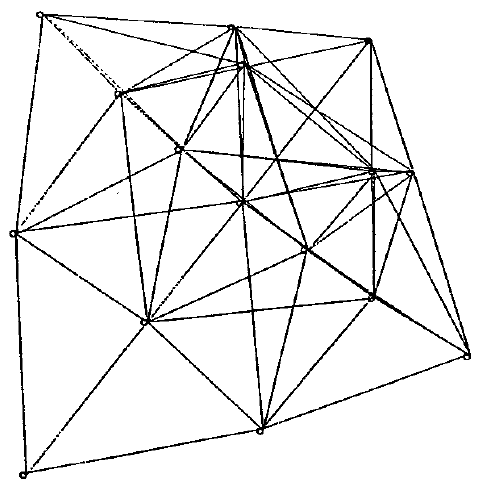
\includegraphics[width=\textwidth]{Eades_dense.png}
\caption[Visualisierung eines dichten Graphen]{Visualisierung eines dichten Graphen, Quelle: \protect\citeA{eades1984heuristic}}
\label{Eades_dense}
\end{subfigure}
\begin{subfigure}[b]{0.45\textwidth}
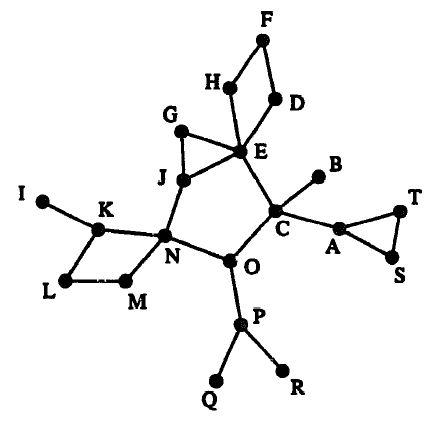
\includegraphics[width=\textwidth]{kamada_kawai_asymmetric_graph.png}
\caption[Visualisierung eines asymmetrischen Graphen]{Visualisierung eines asymmetrischen Graphen, Quelle: \protect\citeA{kamada1989algorithm}}
\label{kamada_kawai_asymmetric_graph}
\end{subfigure}

\begin{subfigure}[b]{0.45\textwidth}
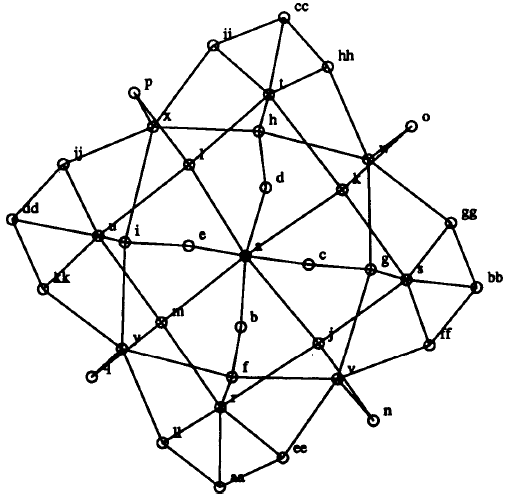
\includegraphics[width=\textwidth]{Fruchterman_Reingold_G1_30sec.png}
\caption[Visualisierung eines Graphen, die in 30 Sekunden berechnet wurde]{Visualisierung eines Graphen, die in 30 Sekunden berechnet wurde, Quelle: \protect\citeA{fruchterman1991graph}}
\label{Fruchterman_Reingold_G1_30sec}
\end{subfigure}
\begin{subfigure}[b]{0.45\textwidth}
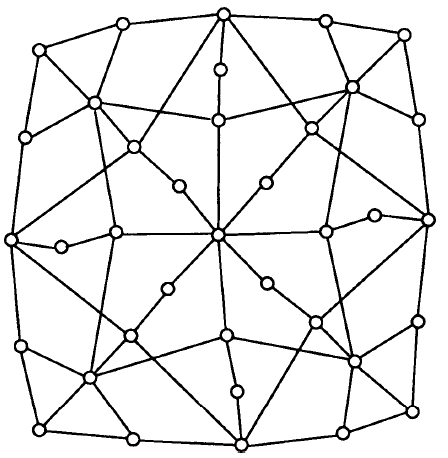
\includegraphics[width=\textwidth]{Davidson_Harel_G1_10min.png}
\caption[Visualisierung eines ästhetischen Graphen, die in 10 Minuten berechnet wurde]{Visualisierung eines ästhetischen Graphen, die in 10 Minuten berechnet wurde, Quelle: \protect\citeA{davidson1996drawing}}
\label{Davidson_Harel_G1_10min}
\end{subfigure}
\caption{Überblick über Ergebnisse verschiedener Visualisierungsalgorithmen für Graphen}
\end{figure}

\newpage
\section{Konzept}
\subsection{Aufbau und Kategorisierung der Wikipedia}
\subsubsection{Übersetzung des Aufbaus der Wikipedia in einen Wissensgraphen}
Die Wikipedia ist eine Datenbank, die ein dichtes Netz aus mehreren Millionen Artikeln bildet \cite{Wiki:02}. Die Einträge in diesem Online-Lexikon beinhalten sowohl im Fließtext als auch in anderen Teilelementen eines Artikels Verweise auf weitere Artikel. Versucht man, Artikel und deren Referenzen untereinander graphisch darzustellen, fällt einem schnell die Ähnlichkeit zu einem mathematischen Graphen auf.\\

\begin{figure}[h!]
\centering
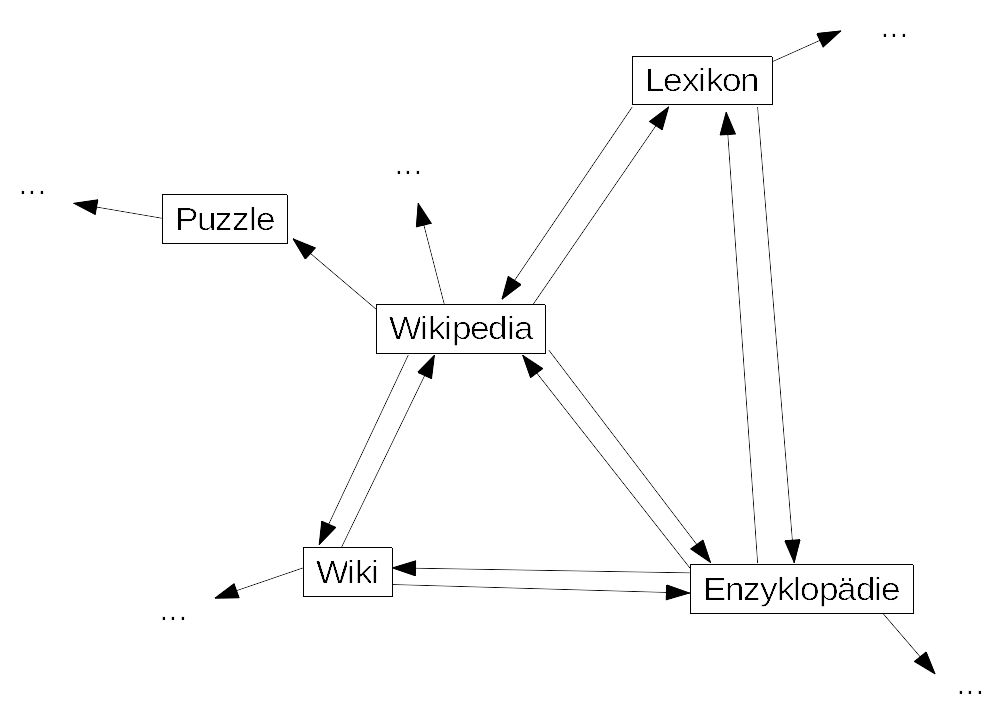
\includegraphics[width=0.95\textwidth]{Ausschnitt_Wikipedia.png}
\caption[Beispielhafter Ausschnitt aus der Wikipedia]{Beispielhafter Ausschnitt aus der Wikipedia (Stand 06.03.2018), eigene Darstellung}
\label{wikiAusschnitt}
\end{figure}

Wie in Abb.~\ref{wikiAusschnitt} zu sehen ist, können Artikel beidseitige Referenzen haben, d.h.  ein Artikel referenziert einen anderen Artikel, der eine Referenz zum ursprünglichen Artikel beinhaltet. Nicht alle Artikel haben allerdings solch eine Beziehung zueinander, Referenzen müssen nicht zurückführen. In Abb.~\ref{wikiAusschnitt} referenziert der Artikel "`Wikipedia"' beispielsweise den Eintrag "`Puzzle"'. Dieser Artikel hat aber keine Referenz zurück.\\

Beziehen wir diese Struktur auf Graphen, so sehen wir, dass die Artikel gut als Knoten modelliert werden können. Die Referenzen zwischen Artikeln bilden gerichtete Kanten. Auch können wir sehen, dass die Wikipedia als Graph modelliert Kreise hat, also zyklisch ist.\\

\subsubsection{Aufführen der einzelnen Elemente eines Wikipedia-Artikels}
Ein einzelner Artikel der Wikipedia kann aus vielen verschiedenen Elementen bestehen und Eigenschaften besitzen. Wichtig zu beachten ist, dass nicht alle Artikel, die auf der Wikipedia zu finden sind, auch tatsächlich alle der im Folgenden aufgeführten Elemente besitzen. Besonders kurze Artikel bestehen häufig nur aus einem eindeutigen Titel, dem Einleitungstext und einer Literaturangabe, wobei diese auch nicht immer vorhanden ist (Beispiel: Artikel "`Liste der Kardinalpriester von San Leone Magno"'). Folgende Teilelemente können neben dem Titel und Einleitungstext in einem Artikel vorkommen:
\begin{description}
\item[Inhaltsverzeichnis] Das Inhaltsverzeichnis eines Artikels wird automatisch erstellt, wenn der Artikel mehr als drei Kapitel hat \protect\cite{wiki:03}. Es wird direkt nach dem Einleitungstext angezeigt und beinhaltet anklickbare Verweise auf die Kapitel des Artikels.
\item[Kapitel] In den Kapiteln eines Artikels stehen detaillierte Informationen zum betrachteten Thema. Es gibt kein festgelegtes Format, nach dem Kollaborateure einen Artikel erstellen oder gliedern müssen. Viele Artikel haben allerdings einen ähnlichen Aufbau, bei dem nach mehreren Kapiteln Inhalt ein paar Kapitel zu Literatur und Nachweisen folgen. Häufig, aber nicht immer, sind die letzten Kapitel "`Siehe auch"', "`Literatur"', "`Weblinks"' und "`Einzelnachweise"'. Der Sinn dieser Kapitel liegt darin, Quellen und relevante Inhalte zum betrachteten Thema aufzuführen.
\item[Eingebettete Mediendateien] Es gibt viele verschiedene Dateien, die in einem Wikipedia Artikel eingebettet werden können. Diese können Vektorgrafiken, Rastergrafiken, Audio oder auch Video sein. Die erlaubten Formate sind online abrufbar \cite{wiki:04}, wobei die wichtigsten Dateitypen für Bilder SVG, PNG, JPEG, GIF und XCF, für Ton OGG-Container und für Videos WebM und OGV sind.
\item[Infobox] Nicht alle Artikel haben eine Infobox, Artikel bestimmter Kategorien werden allerdings immer mit einer Infobox erstellt. Ein Beispiel dafür wären Artikel der Kategorie "`Band"', die am Anfang der Seite standardmäßig eine Infobox mit einem kleinen ergänzenden Überblick über die Band haben. 
\item[Navigationsleiste] Navigationsleisten befinden sich normalerweise unten auf einem Artikel und bieten eine Übersicht über verwandte Artikel. Sie ermöglichen dem Nutzer, schneller zwischen Artikeln aus einem Themengebiet zu navigieren.
\end{description}
Bei der Umsetzung einer Anwendung zur Visualisierung von Artikeln ist es notwendig, alle genannten Elemente und Dateitypen zu berücksichtigen und, falls möglich, dem Anwender präsentieren zu können.\\

\subsubsection{Aufführen der komplexitätsbestimmenden Parameter}
Der Graph, der schließlich aus den einzelnen Artikeln und deren Verbindungen untereinander entsteht, ist sehr groß, dicht und unübersichtlich. Verschiedene Parameter sorgen dafür, dass der Graph leichter oder schwerer zu überblicken ist.\\

Eine ganz zentrale Eigenschaft, die auch später in der Visualisierung des Graphen eine große Rolle spielt, ist die Menge der Knoten. Da die Wikipedia mehr als 2 Millionen enzyklopädische Einträge umfasst und sogar über 6 Millionen Einträge umfasst, wenn man Spezialseiten, wie Nutzerseiten oder Hilfsseiten, dazuzählt, spielt die Anzahl der Knoten eine entscheidende Rolle beim Betrachten und Arbeiten mit dem Graph. Je mehr Knoten der Graph hat, desto unübersichtlicher wird die Visualisierung. Nach\citeA{herman2000graph} leiden bei einem zu großen Graph Anschaulichkeit und Benutzerfreundlichkeit, auch wenn tatsächlich alle Knoten und Kanten dargestellt werden können. Abb. \ref{hermanBigGraph} verdeutlicht, wie ein nicht allzu großer Baum bereits unüberschaubar sein kann. Vor allem in dem hier vorgeschlagenen Konzept ist es wichtig, eine Begrenzung der angezeigten Wikipedia Artikel einzuführen. Da viele Artikel eine hohe Anzahl an Links aufweisen, kann es schnell passieren, dass selbst scheinbar kleine Ausschnitte aus der Wikipedia sehr groß sein können. Ein Beispiel hierfür wäre der Graph den wir bekommen, wenn wir den Artikel "`Mond"' und alle in diesem Artikel referenzierten Nachbarn visualisieren. Dieser Graph hätte bereits 749 Knoten, wobei einer davon der Artikel "`Mond"' ist und die anderen dessen direkte Nachbarn. Diese Zahl rechnet Artikel nicht mit ein, die nicht von "`Mond"' verwiesen werden, aber auf diesen Artikel zeigen. So hätte der Graph zum Eintrag "`Mond"' sogar 2346 Knoten, wenn solche Einträge auch angezeigt werden sollen.\\

\begin{figure}[h!]
\centering
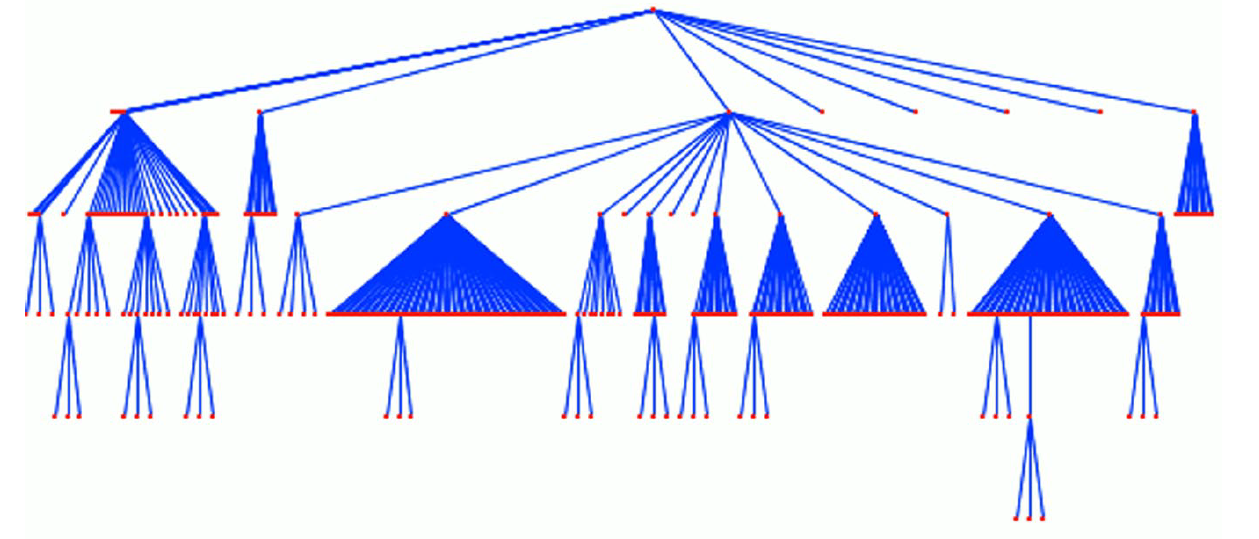
\includegraphics[width=0.95\textwidth]{hermanBigGraph.png}
\caption[Ein mäßig großer Baum]{Ein mäßig großer Baum, Quelle: \protect\citeA{herman2000graph}}
\label{hermanBigGraph}
\end{figure}

Das Problem der außerordentlich großen Menge an Knoten, die man beim Darstellen eines Ausschnitts der Wikipedia betrachtet, wird indirekt auch von einem weiteren Parameter beeinflusst. Dieser ist die Anzahl an Sprünge, die wir von unserem Startknoten aus machen dürfen. Damit ist gemeint, wie weit wir uns vom Startknoten entfernen können und wie lang die kürzesten Wege zwischen dem Startknoten und einem beliebigen anderen Knoten im Graph sein dürfen. Das oben genannte Beispiel geht davon aus, dass wir nur einen Sprung machen dürfen. Das bedeutet, wir nehmen unseren Startknoten und alle Nachbarn dessen in den Graphen mit auf. Wenn wir zwei Sprünge erlauben, müssen wir alle direkten Nachbarn der Nachbarn des Startknotens zusätzlich mit aufnehmen, bei drei Sprüngen auch dessen Nachbarn und so weiter. Da Artikel sehr unterschiedlich viele Referenzen besitzen, ist es schwer einzuschätzen, wie schnell dadurch wiederum die Anzahl an darzustellenden Knoten steigt. Nehmen wir stattdessen an, wir haben eine durchschnittliche Gradzahl
\begin{equation} \label{avgDegree}
avgDegree = \frac{\sum_{i \in V} \enskip deg(i)}{|V|},
\end{equation}
wobei $V$ hier die Knotenmenge aller Wikipedia Artikel repräsentiert. Bezeichnen wir die Anzahl an Sprüngen als $j$ und haben alle betrachteten Artikel $avgDegree$-viele Nachbarn, so ist die Menge an Knoten in einem Ausschnitt aus der Wikipedia
\begin{equation} \label{nodeAmountAvg}
|V_{Ausschnitt}| = 1+avgDegree+\sum_{i=2}^{j} (avgDegree-1)^i
\end{equation}
Zusätzlich nehmen wir hier an, dass alle Nachbarn, bis auf den, über den man erreicht wurde, einzigartig sind und noch nicht "`ausgeklappt"' wurden. Auch wird zur Vereinfachung angenommen, dass alle Nachbarn auch eine Referenz zurück zum aktuellen Knoten haben, wir stellen den Graph also ungerichtet dar. Abb.~\ref{graphJumpsFour} stellt diese Formel für $j=2$ und $avgDegree=4$ dar. Die Einträge in den Ringen entsprechen den Summanden der Formel $1$, $avgDegree$ und $(avgDegree-1)^2$.\\

\begin{figure}[h!]
\centering
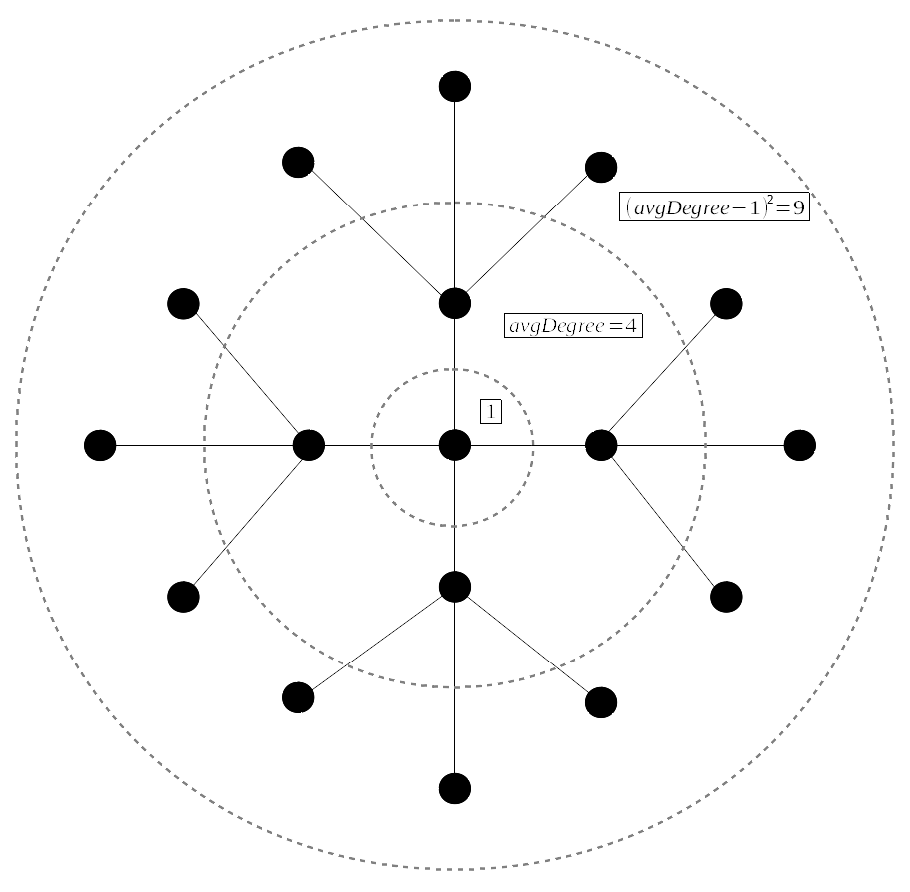
\includegraphics[width=0.95\textwidth]{graphJumpsFour.png}
\caption[Darstellung eines Teilgraphen mit $j=2$ und $avgDegree=4$]{Darstellung eines Teilgraphen mit $j=2$ und $avgDegree=4$, eigene Darstellung}
\label{graphJumpsFour}
\end{figure}

Ein wichtiger Wert in der Visualisierung von Teilgraphen innerhalb der Wikipedia ist demnach auch der Grad eines Knotens. Im Gegensatz zu der dargestellten Menge an Knoten und den Sprüngen, die vom Startknoten aus erlaubt sind, ist dieser Wert allerdings nicht manipulierbar. Er ist durch die Anzahl der Referenzen eines Artikels gegeben und bestimmt dadurch zusammen mit der Anzahl an erlaubten Sprüngen die Menge an Knoten des betrachteten Graphen.\\

\newpage
\subsection{Visualisierung von Artikeln und Verlinkungen in VR}
\subsubsection{Fruchterman-Reingold-Algorithmus im dreidimensionalen Raum}
Der Graph, den wir durch Analyse der Wikipedia erhalten, besteht zwar aus einer Menge von Knoten und Kanten, enthält aber noch keine Informationen zur Darstellung. Um den Graphen darstellen zu können, ist es also nötig, den gefundenen Knoten Positionen zuweisen zu können. Hierfür verwenden wir einen Visualisierungsalgorithmus, der Positionen für die Knoten eines Graphen berechnet.\\

Der Algorithmus von \citeA{fruchterman1991graph} wurde ursprünglich für ungerichtete Graphen im zweidimensionalen Raum formuliert. Abbildung~\ref{frAlg} zeigt den ursprünglichen Pseudocode für den auf Kräften basierenden Algorithmus, wie er von Fruchterman und Reingold vorgestellt wurde.\\

\begin{algorithm}
	\caption{Fruchterman-Reingold-Algorithmus, adaptiert aus \protect\citeA{fruchterman1991graph}}\label{frAlg}
	\begin{algorithmic}
	\State $area:=W*L$; \{W and L are the width and length of the frame\}
	\State $G:=(V,E)$; \{the vertices are assigned random initial positions\}
    \State $k:=\sqrt{area/|V|}$;
    \State \textbf{function} $f_a(z) :=$ \textbf{begin return} $z^2/k$ \textbf{end};
    \State \textbf{function} $f_r(z) :=$ \textbf{begin return} $k^2/z$ \textbf{end};
    \For{$i:=1$ \textbf{to} iterations}
    	\State \{calculate repulsive forces\}
        \For{$v \in V$}
        	\State \{each vertex has two vectors: .pos and .disp\}
            \State $v.disp := 0$;
            \For{$u \in V$}
            	\If{$u \neq v$}
                	\State \{$\Delta$ is short hand for the difference\}
                    \State \{vector between the positions of the two vertices\}
                    \State $\Delta := v.pos - u.pos$;
                    \State $v.disp := v.disp + (\Delta / |\Delta|) * f_r(|\Delta|)$;
                \EndIf
            \EndFor
        \EndFor
        \State \{calculate attractive forces\}
        \For{$e \in E$}
        	\State \{each edge is an ordered pair of vertices .v and .u\}
            \State $\Delta := e.v.pos - e.u.pos$
            \State $e.v.disp := e.v.disp - (\Delta / |\Delta|) * f_a(|\Delta|)$;
            \State $e.u.disp := e.u.disp + (\Delta / |\Delta|) * f_a(|\Delta|)$;
        \EndFor
        \State \{limit the maximum displacement to the temperature t\}
        \State \{and then prevent from being displaced outside frame\}
        \For{$v \in V$}
        	\State $v.pos := v.pos + (v.disp / |v.disp|) * min(|v.disp|, t)$;
            \State $v.pos.x := min(W/2, max(-W/2, v.pos.x))$;
            \State $v.pos.y := min(L/2, max(-L/2, v.pos.x))$;
        \EndFor
        \State \{reduce the temperature as the layout approaches a better configuration\}
        \State $t := cool(t)$;
    \EndFor
	\end{algorithmic}
\end{algorithm}

Um ihn in einer virtuellen Welt verwenden zu können, muss der vorgestellte Pseudocode erst angepasst werden. In der originalen Fassung wird eine Fläche aus Breite und Höhe des verfügbaren Rahmens berechnet, in welchem der Graph gezeichnet werden soll. Die verwendete Formel für die Fläche ist im zweidimensionalen Raum
\begin{equation} \label{areaTwoDim}
area = W * L,
\end{equation}
wobei $W$ die Breite und $L$ die Länge des verfügbaren Rahmens ist. Aus dieser Fläche berechnet sich eine optimale Distanz $k$ zwischen zwei Knoten. Diese Distanz wird zur Berechnung der Kräfte zwischen den einzelnen Knotenpaaren verwendet. Die Formel für $k$ ist im Zweidimensionalen
\begin{equation} \label{optimalKTwoDim}
k = C * \sqrt{area / |V|},
\end{equation}
wobei $V$ die Menge der zu zeichnenden Knoten ist. Im Algorithmus selber wird die Konstante $C$ allerdings weggelassen. Passen wir Formel \eqref{areaTwoDim} an einen dreidimensionalen Raum an, so bekommen wir
\begin{equation} \label{volumeThreeDim}
volume = W * L * H.
\end{equation}
Diese Formel berechnet allerdings ein Volumen mithilfe der zusätzlichen Höhe $H$. Die Fläche im originalen Algorithmus wird zur Berechnung von $k$ verwendet. In Formel \eqref{optimalKTwoDim} wird diese Fläche durch die Anzahl der Knoten im Graphen geteilt und aus diesem Wert anschließend die Wurzel gezogen. Der Ausdruck $area/|V|$ gibt uns eine durchschnittliche Fläche, die pro Knoten verfügbar ist. Wenn wir einen Gittergraphen betrachten, in dem alle Knoten gleich verteilt sind und den gleichen Abstand (nämlich $k$) zu ihren direkten Nachbarn haben, können wir uns diese Fläche besser vorstellen. Abb.~\ref{gridGraphOptimalDistance} zeigt einen Gittergraphen, wobei allen Knoten eine gleich große quadratische Fläche zugeordnet werden kann.\\

\begin{figure}[h!]
\centering
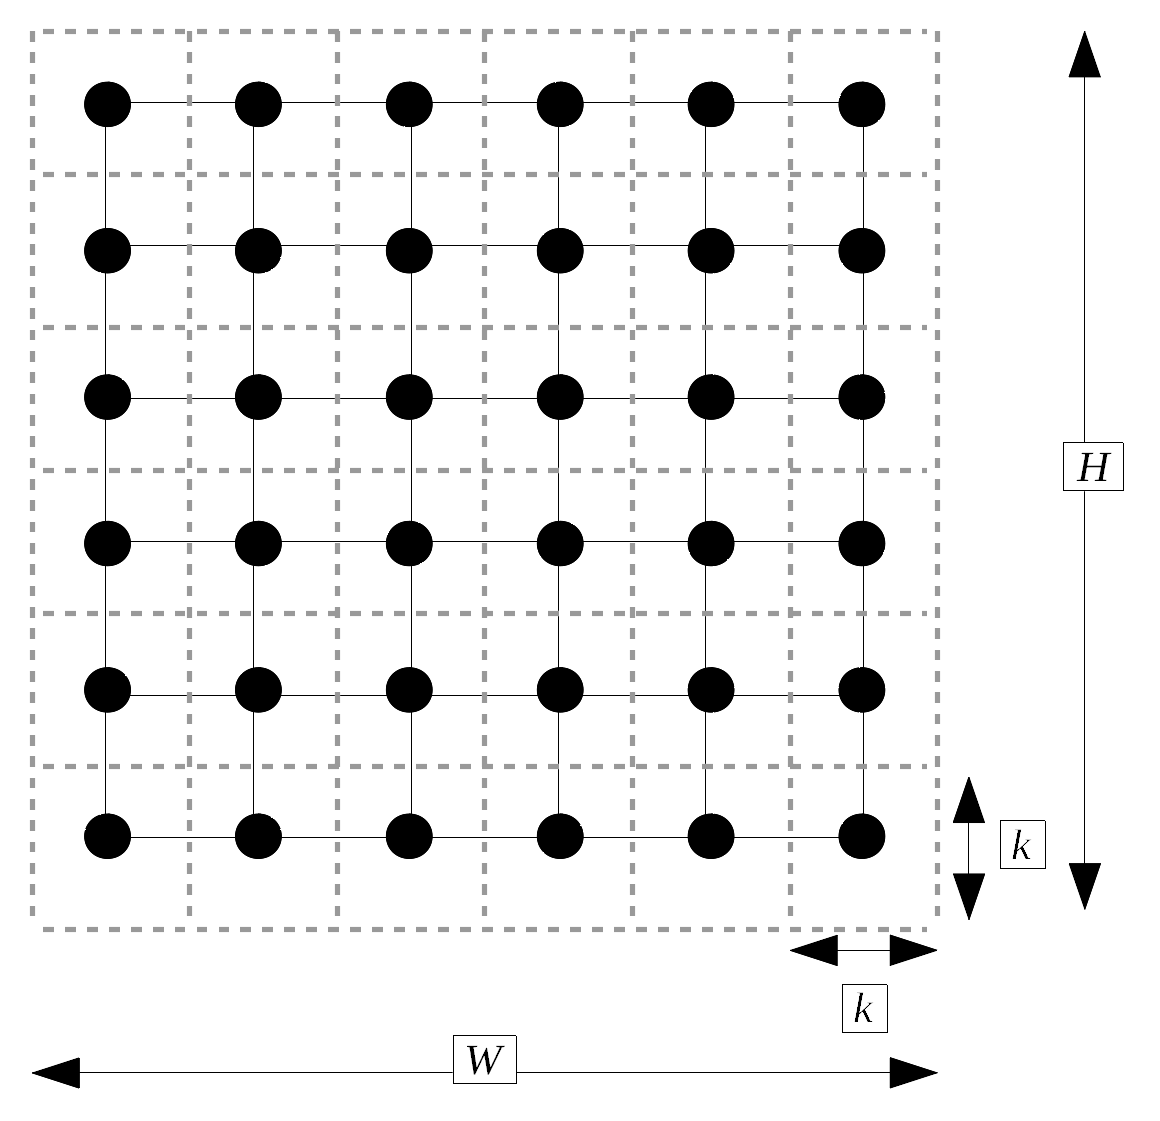
\includegraphics[width=0.95\textwidth]{gridGraphOptimalDistance.png}
\caption[Ein Gittergraph mit Breite $W$,  Höhe $H$ und $|V|=36$]{Ein Gittergraph mit Breite $W$,  Höhe $H$ und $|V|=36$, eigene Darstellung}
\label{gridGraphOptimalDistance}
\end{figure}

Die besagten Flächen sind in Abb.~\ref{gridGraphOptimalDistance} durch die grauen, gestrichelten Linien dargestellt. Unschwer zu erkennen ist, dass hier jede Fläche $area_{node} = (W*H)/|V| = (W*H)/36$ groß ist. Dieser Wert $area_{node}$ ist genau derjenige, der in Formel \eqref{optimalKTwoDim} in der Wurzel steht. Das in Abb.~\ref{gridGraphOptimalDistance} eingezeichnete $k$ gilt dabei für $C=1$. Tatsächlich ist dies aber nicht der optimale Wert für $k$, da nur $\frac{5}{6}*\frac{5}{6} \approx 69,44\%$ der verfügbaren Fläche ausgenutzt wird. Wir können den Gittergraphen um $\frac{1}{2}k$ nach links und um $\frac{1}{2}k$ nach oben verschieben und haben so freie Flächen am unteren und rechten Rand. Zudem kommt, dass nicht alle Graphen perfekt als Gittergraphen dargestellt werden können.\\

Fügen wir dem Graphen und dem Gitter in Abb.~\ref{gridGraphOptimalDistance} eine Dimension hinzu, werden aus den quadratischen Flächen Würfel mit der Seitenlänge $k$. Hier ergibt sich auch die zugehörige Anpassung der Formel für $k$, nämlich
\begin{equation} \label{optimalKThreeDim}
k =\sqrt[3]{volume/|V|}.
\end{equation}
Wir ziehen nun die Kubikwurzel aus dem verfügbaren Raum pro Knoten, um die Seitenlänge $k$ zu bekommen. Das Volumen, welches wir mit dieser Distanz zum nächsten Knoten ausnutzen, ist nun $\frac{5}{6}*\frac{5}{6}*\frac{5}{6} \approx 57,87\%$ des verfügbaren Volumens. Diese Zahl kann durch ein passend gewähltes $C$ verbessert werden.\\

Eine weitere Anpassung, die für eine dreidimensionale Version des Algorithmus durchgeführt werden muss, ist die Mitbeachtung von Werten der dritten Dimensionsachse. Dies bedeutet, dass wir alle Verschiebungs- und Positionsvektoren für drei anstatt für zwei Werte berechnen.\\

\subsubsection{Steigerung der Effizienz des vorgestellten Algorithmus}
Der im vorherigen Abschnitt vorgestellte Algorithmus berechnet alle abstoßenden Kräfte in Abhängigkeit aller verfügbaren Knoten und dann alle anziehenden Kräfte mit Hilfe der Kantenliste. Dadurch hat er eine Komplexität von $O(|V|^2 + |E|)$. Die Berechnung der anziehenden Kräfte ist hierbei der Term $O(|E|)$, welcher bereits eine Vereinfachung der Realität ist. Hier werden nur Kräfte zwischen Knoten ausgerechnet, die tatsächlich direkt miteinander verbunden sind. Die Berechnung der abstoßenden Kräfte ist hingegen quadratisch. Für kleinere Graphen ist dies kein Problem, doch falls der Anwender einen besonders großen Graphen ansehen möchte, kann die Laufzeit des Algorithmus sehr hoch werden und dadurch die Verfügbarkeit eines Ergebnisses für die Anwendung in Echtzeit zu spät sein.  Da die Berechnung der Knotenpositionen nicht perfekt sein muss um gute Ergebnisse zu liefern, lässt sich der Algorithmus allerdings etwas optimieren.\\

\citeA{fruchterman1991graph} stellen hierfür für Ihren zweidimensionalen Algorithmus eine "`grid-based"' (also gitterbasierte) Variante vor. Nach \citeA{fruchterman1991graph} sinkt die abstoßende Kraft zwischen zwei Knoten mit dem inversen Quadrat der Distanz zwischen ihnen, womit weiter entfernte Knoten weniger ins Gewicht fallen und somit ohne große Verluste ignoriert werden dürfen. Für die gitterbasierte Anpassung werden die Knoten des Graphen pro Iterationsschritt anhand ihrer Position im Gitter in Bereiche eingeordnet. Diese Bereiche sind gleichgroße Quadrate, ähnlich wie in Abb.~\ref{gridGraphOptimalDistance}, wobei die Seitenlänge eines Quadrats $s=2k$ ist. Abstoßende Kräfte werden nun nicht mehr zwischen allen Knotenpaaren berechnet, sondern nur noch zwischen Paaren, die innerhalb des gleichen Bereichs oder adjazenten Bereichen liegen. Diese Anpassung liefert nach \citeA{fruchterman1991graph} allerdings verzerrte Ergebnisse, weswegen zusätzlich eine zweite Bedingung eingeführt wird. Knoten, die die abstoßenden Kräfte am aktuell betrachteten Knoten beeinflussen können, müssen innerhalb eines Radius $r=2k$ des betrachteten Knoten liegen.\\

Die Formel für die abstoßenden Kräfte ist damit
\begin{equation} \label{repForceU}
f_r = \frac{k^2}{d}*u(2k-d),
\end{equation}
wobei
\begin{equation} \label{uFunction}
u(x) = \begin{cases} 1, \quad falls \quad x>0 \\ 0, \quad sonst \end{cases}
\end{equation}
Abb.~\ref{fruchtermanReingoldGridBased} veranschaulicht die Unterteilung der verfügbaren Fläche in gleichgroße Quadrate mit Seitenlänge $s=2k$.\\

\begin{figure}[h!]
\centering
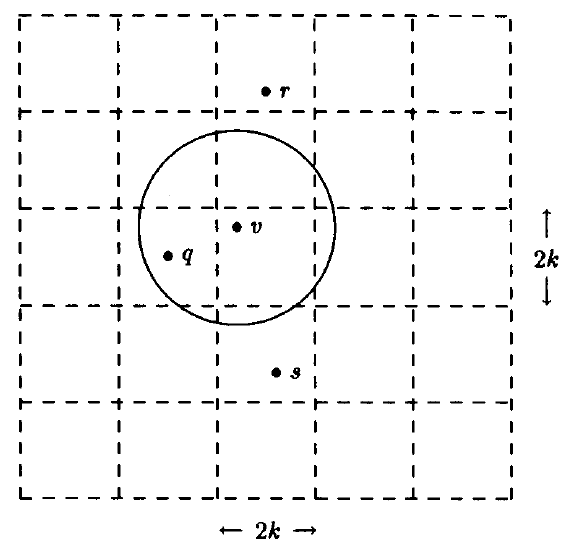
\includegraphics[width=0.95\textwidth]{fruchtermanReingoldGridBased.png}
\caption[Graph mit gitterbasierter Unterteilung]{Graph mit gitterbasierter Unterteilung, Quelle: \protect\citeA{fruchterman1991graph}}
\label{fruchtermanReingoldGridBased}
\end{figure}

In der Umgebung von Knoten $v$ befinden sich zwei Knoten, die für eine Berechnung von abstoßenden Kräften in Frage kommen, nämlich $q$ und $s$. Der Knoten $r$ hingegen liegt nicht in einem zu $v$ adjazenten Bereich. Da $s$ aber nicht in einem Radius von $2k$ um $v$ liegt, fällt dieser Knoten für die Berechnung weg. Nur noch $q$ wird im Beispiel aus Abb.~\ref{fruchtermanReingoldGridBased} für den Knoten $v$ zur Berechnung von abstoßenden Kräften beachtet.\\

Die Fläche, in dem Knoten die abstoßenden Kräfte eines gewählten Knoten beeinflussen können, ist, wie auch im ursprünglichen Algorithmus zur Berechnung von $k$ verwendet wird,
\begin{equation}
A = \frac{W*L}{|V|},
\end{equation}
wobei $k$ auch hier wieder die Wurzel dessen ist, also
\begin{equation}
k = \sqrt{A}.
\end{equation}
Wenn nun die Seitenlänge eines Gitterbereichs $s=2k$ ist, so lässt sich mit diesen Werten auch die Anzahl der benötigten Gitterbereiche berechnen:
\begin{equation}
|Gitterbereiche| = \frac{W}{2k}\frac{L}{2k} = \frac{WL}{4k^2} = \frac{WL}{4\frac{WL}{|V|}} = \frac{WL*|V|}{4WL} = \frac{|V|}{4}
\end{equation}

Wenn die Verteilung der Knoten des Graphen im Raum etwa gleichmäßig ist, so verringert sich die Komplexität der Berechnung abstoßender Kräfte im gesamten Graphen auf $\Theta(|V|)$ \cite[S.~1137]{fruchterman1991graph}.\\

Für die Übersetzung der genannten Formeln in eine dreidimensionale Umgebung ist kein großer Aufwand notwendig. Statt der Fläche $A$ berechnen wir ein Volumen $V$, welches pro Knoten verfügbar ist
\begin{equation}
V = \frac{WLH}{|V|}.
\end{equation}
Das zugehörige k ist nun
\begin{equation}
k = \sqrt[3]{V}.
\end{equation}
Die Berechnung der Anzahl an Gitterboxen ist auch äquivalent:
\begin{equation} \label{gridBoxes3D}
\frac{W}{2k}\frac{L}{2k}\frac{H}{2k} = \frac{WLH}{8k^3} = \frac{|V|}{8}.
\end{equation}

\subsubsection{Bedeutung der Kantenrichtungen für Algorithmus und Darstellung}
Der vorgestellte Algorithmus von Fruchterman und Reingold wird angewendet, um ungerichtete Graphen darzustellen. Für die Visualisierung eines Teilausschnittes aus der Wikipedia werden Kanten aber mit Richtungen modelliert. Um den Algorithmus nach wie vor auf den gegebenen Graphen anwenden zu können, muss dieser wie ein ungerichteter Graph behandelt werden.\\

Da der ausgewählte Algorithmus als Eingabe eine Knotenliste und eine Kantenliste erwartet, kann die Kantenliste so modelliert werden, dass Informationen über die Richtung einer Kante in dieser abgespeichert werden. Ein Eintrag in der Kantenliste besteht dann aus einer Information bei welchem Artikel die Kante anfängt (also der Wikipedia Eintrag, der den Link enthält) und zu welchem Artikel sie führt (der Eintrag, der beim folgen des Links erreicht wird). Zusätzlich wird ein Wert gespeichert, der bestimmt, ob die Kante gegenläufig ist, also in beide Richtungen zeigt.\\

Bei der Berechnung anziehender Kräfte zwischen Knoten wird dann die Kantenliste durchlaufen und jede eingetragene Kante so behandelt, als wäre sie gegenläufig. Der Algorithmus behandelt den Graphen also als ungerichtet und vereinfacht gerichtete Kanten zu gegenläufigen Kanten. In Abb.~\ref{exampleMondDirection} ist ein echter Teilausschnitt der Wikipedia dargestellt, mit dem Artikel "`Mond"' als Startknoten. In Abb.~\ref{exampleMondNoDirection_noLabels} ist der gleiche Graph aber mit ungerichteten Kanten zu sehen. Der Algorithmus behandelt den Graphen nicht wie in Abb.~\ref{exampleMondDirection}, sondern wie in Abb.~\ref{exampleMondNoDirection_noLabels}.\\

\begin{figure}[h!]
\centering
\begin{subfigure}[t]{0.55\textwidth}
\centering
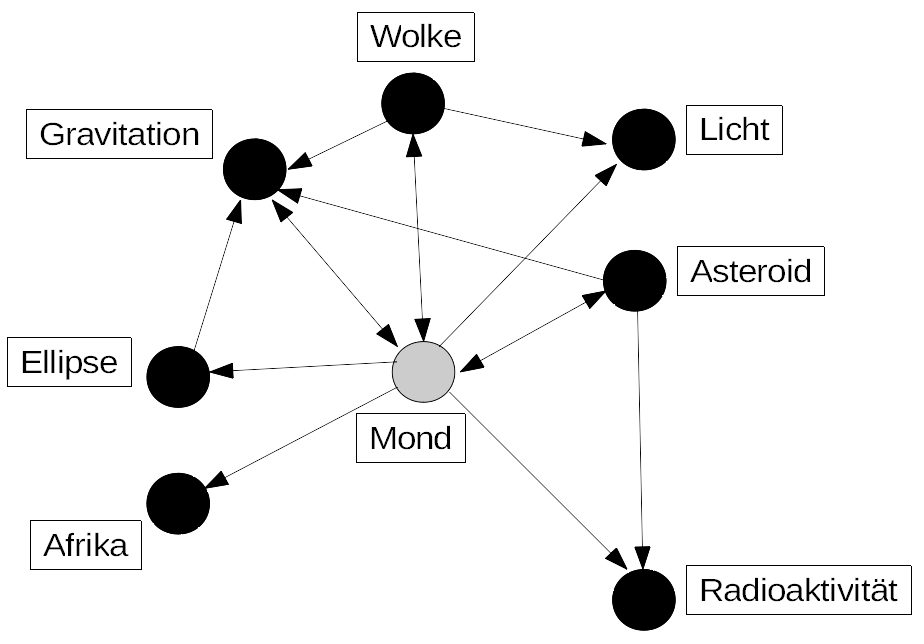
\includegraphics[width=0.95\textwidth]{exampleMondDirection.png}
\caption[Teilgraph der Wikipedia mit Informationen über Linkrichtungen]{Teilgraph der Wikipedia mit Informationen über Linkrichtungen, eigene Darstellung}
\label{exampleMondDirection}
\end{subfigure}\hfill
\begin{subfigure}[t]{0.35\textwidth}
\centering
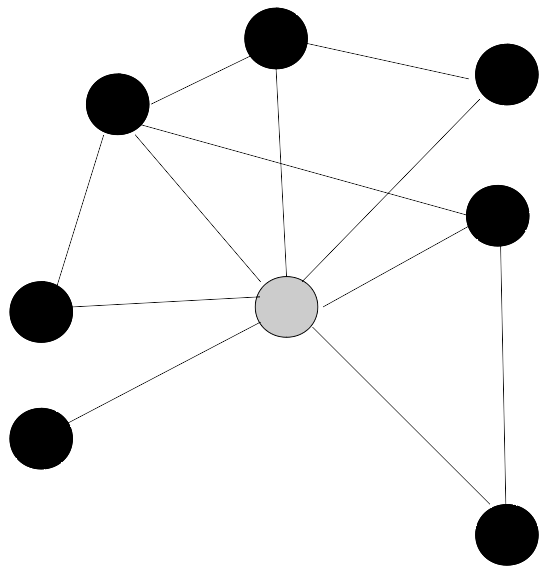
\includegraphics[width=0.95\textwidth]{exampleMondNoDirection_noLabels.png}
\caption[Teilgraph der Wikipedia, wie er vom Algorithmus behandelt wird]{Teilgraph der Wikipedia, wie er vom Algorithmus behandelt wird, eigene Darstellung}
\label{exampleMondNoDirection_noLabels}
\end{subfigure}
\caption{Ausschnitt der Wikipedia wie er dargestellt werden soll und wie er für den ausgewählten Visualisierungsalgorithmus behandelt wird.}
\label{exampleMond}
\end{figure}

Das Darstellen des Graphen erfolgt erst nach der Berechnung der Knotenpositionen. Die Richtungen, die in den Einträgen der Kantenlisten angegeben sind, werden hier beim Zeichnen der Kanten mitbeachtet.\\
\newpage
\subsection{Visualisierung von einzelnen Artikeln in VR}
\subsubsection{Darstellung der Teilelemente eines Artikels in VR}
In Kapitel 3.1.2 werden die verschiedenen möglichen Elemente eines Wikipediaartikels aufgeführt. Beim Auswählen eines Knotens in der Darstellung des Graphen soll es möglich sein, sich den durch diesen repräsentierten Artikel anzeigen zu lassen. Da die Visualisierung des Graphen in drei Dimensionen erfolgt und der Nutzer auch dreidimensionale Eingaben machen kann, werden die Bestandteile eines Artikels nicht so angezeigt, wie es in einem Browser zu sehen wäre. Stattdessen werden sie aufgeteilt und getrennt dargestellt. Die einzelnen Elemente werden hierfür auf Flächen projiziert, die wie bedruckte Blätter aussehen und im Raum fixiert werden. Abb. \ref{articleInVR} soll dieses Konzept verdeutlichen. Die einzelnen Elemente des Artikels werden hier nicht zweidimensional im Text eingebettet, anders als auf einem Bildschirm. Dieses Konzept soll vermeiden, den Nutzer mit Informationen zu überwältigen, die er nicht nach Belieben ausblenden kann.\\

\begin{figure}[h!]
\centering
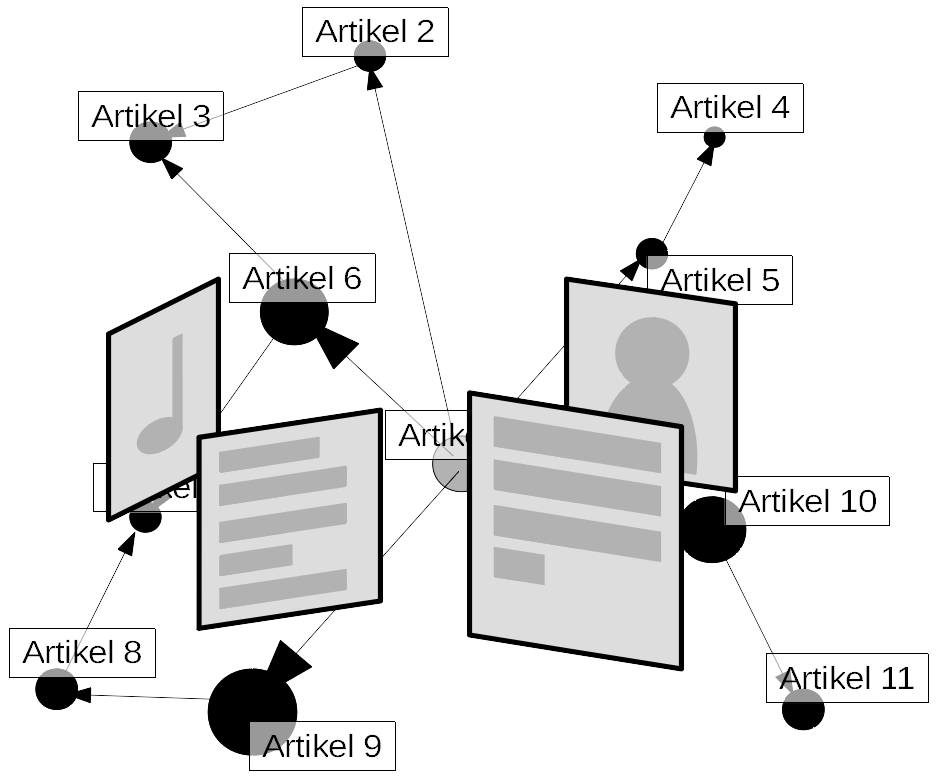
\includegraphics[width=0.95\textwidth]{articleInVR.png}
\caption[Darstellung einzelner Informationen eines Wikipediaartikels im Raum]{Darstellung einzelner Informationen eines Wikipediaartikels im Raum, eigene Darstellung}
\end{figure}

Beim Betrachten eines Wikipediaartikels im Browser lassen sich Bilder häufig auf Spezialseiten zurückverfolgen, auf denen eventuell weitere Auflösungen verfügbar sind. Ein Beispiel hiervon ist das Logo der Technischen Universität München, welches auf der Wikipediaseite mit dem gleichen Namen angezeigt wird und auf einer weiteren Spezialseite in verschiedenen Auflösungen und Formaten verfügbar ist \cite{wiki:TUMlogo}. Dem Nutzer wird im vorgestellten Konzept allerdings nicht die Möglichkeit gegeben, diese Inhalte weiterzuverfolgen, da die konzipierte Anwendung nicht wie ein Browser funktioniert und der Nutzer nicht ohne weiteres verschiedene Webseiten und Quellen verwalten kann. Stattdessen werden alle Bilder und andere Meiden auf eine festgelegte Größe begrenzt oder hochskaliert.\\

Videos im virtuellen Raum werden genau so dargestellt, wie Bilder, nur dass sie zusätzlich die Möglichkeit bieten, abgespielt oder angehalten zu werden. Zusätzlich wird dem Nutzer ein Slider zum Einstellen der Audiolautstärke bereitgestellt. Audioquellen werden wie Videos behandelt, nur dass sie statt einem visuellen Inhalt entweder ein Wiedergabezeichen oder ein Pausenzeichen anzeigen, je nachdem ob die Audioquelle gerade abgespielt wird oder nicht.\\

Bei der Darstellung des Wikipediaartikels in seinen Bausteinen kann der Nutzer über ein Menü zusätzlich auswählen, ob der Graph, in dem er sich gerade befindet, angezeigt werden soll oder nicht. Dies soll der Übersichtlichkeit dienen, falls ein besonders dichter Graph dargestellt wird, dessen Kanten die Betrachtung des Artikels stören oder sogar einzelne Elemente schneidet.\\

\subsubsection{Darstellung der Struktur eines Artikels in VR}

Genauso, wie die Wikipedia als Graph dargestellt werden kann, lässt sich auch ein einzelner Artikel innerhalb der Wikipedia als Graph darstellen. Die Artikel der Wikipedia weisen immer eine Struktur auf, selbst, wenn der Artikel außer Text keine Medien enthält. Die meisten Artikel weisen allerdings eine Struktur aus Kapiteln und Unterkapitel auf.  Eine Visualisierung als Graph kann nun erfolgen, indem ein abstrakter Knoten, der den kompletten Artikel repräsentiert, modelliert wird. Von diesem aus können alle Kapitel als einzelne Knoten erreicht werden. Bestehen einzelne Kapitel aus Unterkapiteln, kann das übergeordnete Kapitel ebenfalls als abstrakter Knoten dargestellt werden, welches wiederum auf die Unterkapitel verweist. Falls es weitere Ebenen in der Struktur der Kapitel gibt, kann dieses Prinzip bis zur tiefsten Ebene weitergeführt werden. So entsteht ein Graph wie in Abb.~\ref{wish_you_were_here}. Der Knoten, der den kompletten Artikel repräsentiert, wird hier grau dargestellt.\\

\begin{figure}
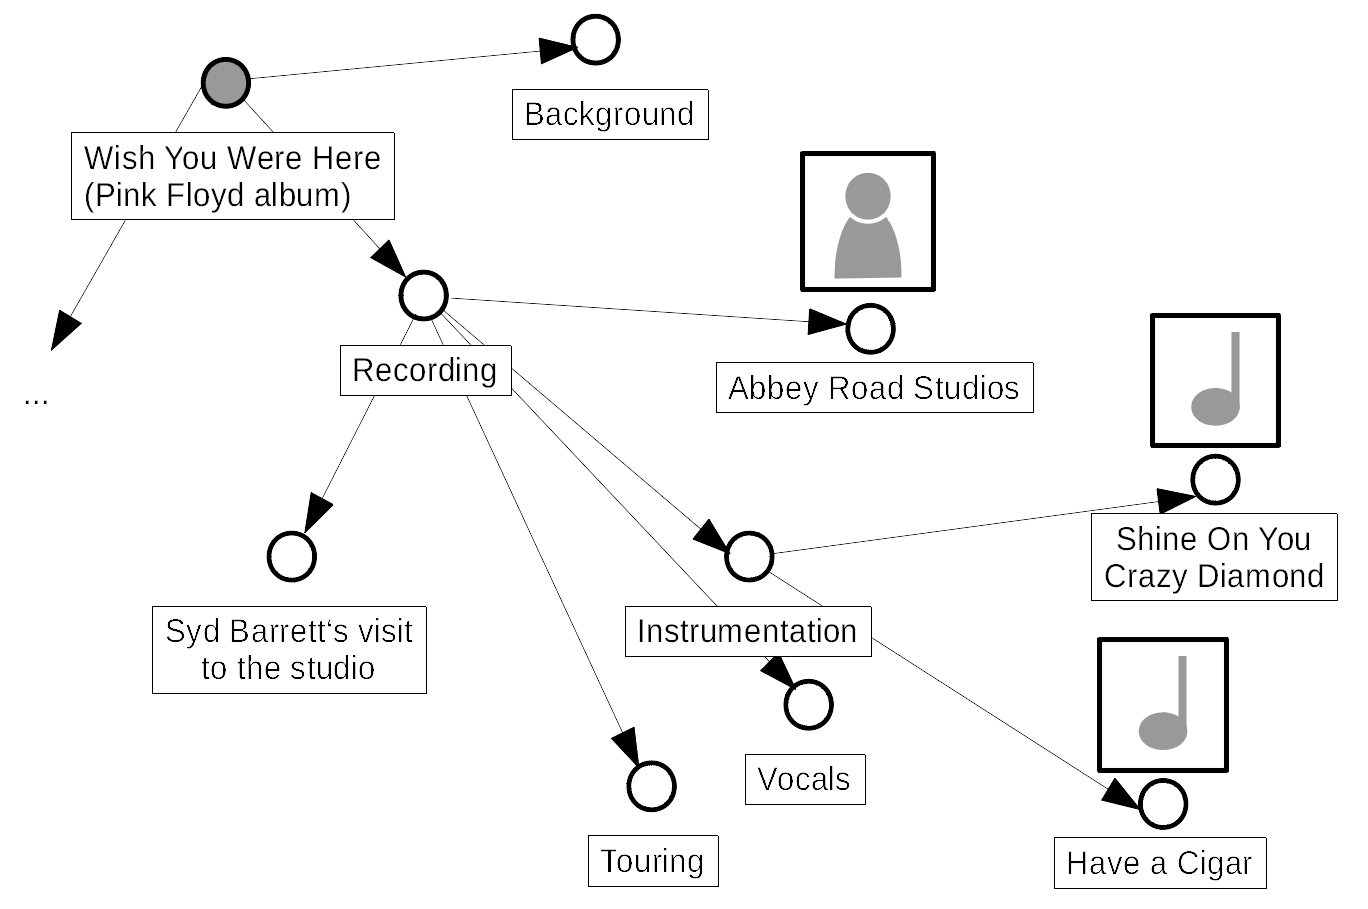
\includegraphics[width=0.9\textwidth]{wish_you_were_here.png}
\caption[Ausschnitt des Graphen zur Struktur des englischen Wikipedia Artikels "`Wish You Were Here (Pink Floyd Album)"']{Ausschnitt des Graphen zur Struktur des englischen Wikipedia Artikels "`Wish You Were Here (Pink Floyd Album)"', eigene Darstellung}
\label{wish_you_were_here}
\end{figure}

An Abb.~\ref{wish_you_were_here} ist zudem die Struktur des Graphen ersichtlich.  Die Knoten, von denen aus kein weiterer Knoten mehr erreichbar ist, sind die im Artikel eingebetteten Medien. Alle Knoten, die auf weitere Knoten zeigen, sind entweder die Repräsentation des Artikels selbst oder Kapitel in diesem. Diese können allerdings auch Textinhalte haben, wie beispielsweise der Einleitungstext des Artikels. Würde der Artikel nur aus einem Einleitungstext bestehen, hätte der zugehörige Graph nach dieser Struktur nur einen Knoten, nämlich der, der den Artikel und den zugehörigen Einleitungstext repräsentiert.\\

Bei der Darstellung der Struktur eines Wikipediaartikels als Graph wird der zugrundeliegende Graph, der die Artikel der Wikipedia repräsentiert, ausgeblendet. Auch dies soll wieder der Übersichtlichkeit dienen.\\

Anders als bei dem Graphen zur Wikipedia hat der Nutzer bei der Visualisierung des Strukturgraphen eines Artikels nicht die Möglichkeit, Parameter einzustellen. Dies liegt daran, dass beim Betrachten eines Artikels alle Informationen, die vom Server bereitgestellt werden können, lokal gespeichert werden und damit keine erneuten Anfragen an den Server gestellt werden müssen. Zudem bestehen selbst längere Artikel aus wenigen einzelnen Bausteinen, verglichen zum Graph der Wikipedia. Der Artikel, der in Abb.~\ref{wish_you_were_here} teilweise als Graph dargestellt wird, hat beispielsweise fünf Bilder, 22 Kapitelüberschriften (einschließlich aller Unterkapitel) und zwei Audiobeispiele. Daraus ergeben sich, zusammen mit dem Knoten, der den Artikel repräsentiert, 30 Knoten. Sollen noch weitere Einzelteile des Artikels veranschaulicht werden, wie beispielsweise das Inhaltsverzeichnis, steigt diese Zahl.\\

\newpage
\subsection{Traversierung des gezeichneten Graphen und darin enthaltener Informationen in VR}
\subsubsection{Berechnung neuer Teilabschnitte eines Graphen}
Um dem Nutzer einer interaktiven Visualisierungssoftware ermöglichen zu können, sich frei im Raum zu bewegen und den betrachteten Graphen durchzugehen, muss der dargestellte Graph immer aktualisiert werden, wenn der Nutzer den Fokus auf einen neuen Artikel setzt. Er soll die Möglichkeit haben, jeden dargestellten Knoten auszuwählen und sich in Echtzeit die zugehörigen Nachbarn anzeigen zu lassen. Damit dies möglich ist, müssen mehrere Aspekte dieser Funktion beachtet werden.\\

Wenn der Nutzer einen Knoten im Graph auswählt, der nicht der aktuelle Knoten ist, verändert sich die Knotenliste des Graphen. Nur Knoten, die die gegebenen Parameter in Abhängigkeit des neuen Startknoten erfüllen, werden beibehalten. In Abb.~\ref{expandingNewNode} ist ein gerichteter Graph dargestellt, in dem ein neuer Knoten ausgewählt wurde. Ausgefüllte Knoten sind vom ursprünglichen Startknoten aus erreichbar, schraffierte Knoten kommen durch die Neuauswahl hinzu. Im Graphen gibt es nun fünf verschiedene Arten an Knoten:
\begin{enumerate}
\item Der ursprüngliche Startknoten
\item Der neu ausgewählte Startknoten
\item Die Knoten, die nur vom ursprünglichen Startknoten aus erreichbar waren
\item Die Knoten, die nur vom neu ausgewählten Startknoten aus erreichbar sind
\item Die Knoten, die sowohl vom ursprünglichen als auch vom neu ausgewählten Startknoten aus erreichbar sind
\end{enumerate}

\begin{figure}[h!]
\centering
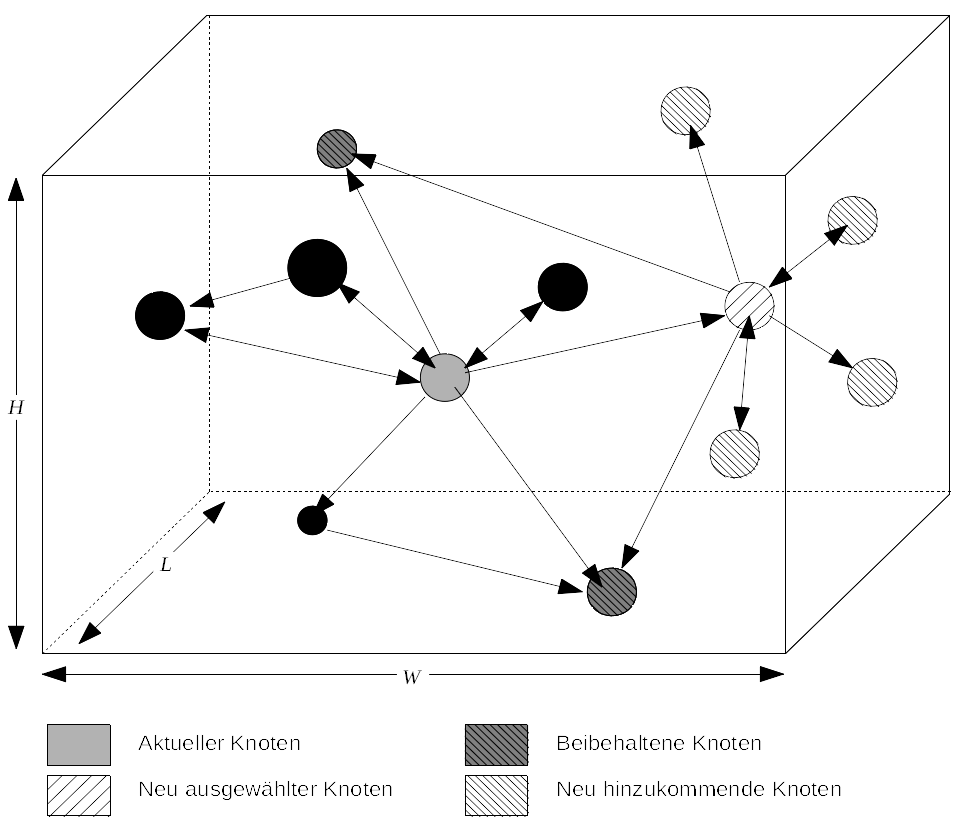
\includegraphics[width=0.95\textwidth]{expandingNewNode.png}
\caption[Beispielhafter Teilausschnitt aus der Wikipedia]{Beispielhafter Teilausschnitt aus der Wikipedia, eigene Darstellung}
\label{expandingNewNode}
\end{figure}

Alle Knoten, die in Abb.~\ref{expandingNewNode} nicht schraffiert sind, werden aus der Knotenliste der Graphen entfernt. Dieser Schritt muss in Abhängigkeit des in Kapitel 3.1.3 erwähnten Sprungparameters erfolgen. Wir führen vom neuen Startknoten aus eine Breitensuche durch und gehen so viele Schritte, wie der Parameter es erlaubt. Alle Knoten die durch diese Suche entdeckt werden, gehören zum neuen Graphen und bekommen eine zufällige Position zugeteilt, um den Visualisierungsalgorithmus ausführen zu können. Knoten, die zuvor in der Knotenliste eingetragen waren und nicht entdeckt werden, werden entfernt. Das gleiche passiert auch mit der Kantenliste.\\

Da sowieso alle Knoten mit der Breitensuche durchlaufen werden müssen, die vom neuen ausgewählten Knoten erreicht werden, kann für diesen Schritt darauf verzichtet werden, die Kantenliste zu behalten. Stattdessen wird eine neue Liste erstellt. Bei der Liste der Knoten ist es möglich, die Knoten zu behalten, die immer noch erreicht werden können. Der Vorteil daran ist, dass bereits visualisierte Knoten eine Position durch Anwenden des Fruchterman-Reingold-Algorithmus aus Kapitel 3.2.1 haben. Andererseits werden diese Positionen durch neues Iterieren über den Algorithmus mit zufällig verteilten neuen Knoten sowieso verändert.\\

Dieser Vorschlag zur Neuberechnung von Teilausschnitten aus dem Graphen, der die Wikipedia darstellt, ist zusätzlich mit der gitterbasierten Variante des Fruchterman-Reingold-Algorithmus aus Kapitel 3.2.2 kompatibel. Der Raum, in dem der Graph gezeichnet werden soll, kann beibehalten werden und neue Knoten dort hineingesetzt werden. Mit den gleichen Werten des Raums kann dann die neue Anzahl an benötigten Gitterboxen und der optimalen Distanz zwischen zwei Knoten $k$ berechnet werden. Abb.~\ref{changeOfGraphOverTime} verdeutlicht, welche Schritte bei der Neuberechnung der Visualisierung eines Teilgraphen ablaufen. Unerreichbare Knoten werden gelöscht und da in Abb.~\ref{graphTraversing_new} $|V|=19$, haben wir schließlich $4 < |Gitterboxen| = \frac{19}{4} < 5$.\\

\begin{figure}
\centering
\begin{subfigure}[t]{0.45\textwidth}
\centering
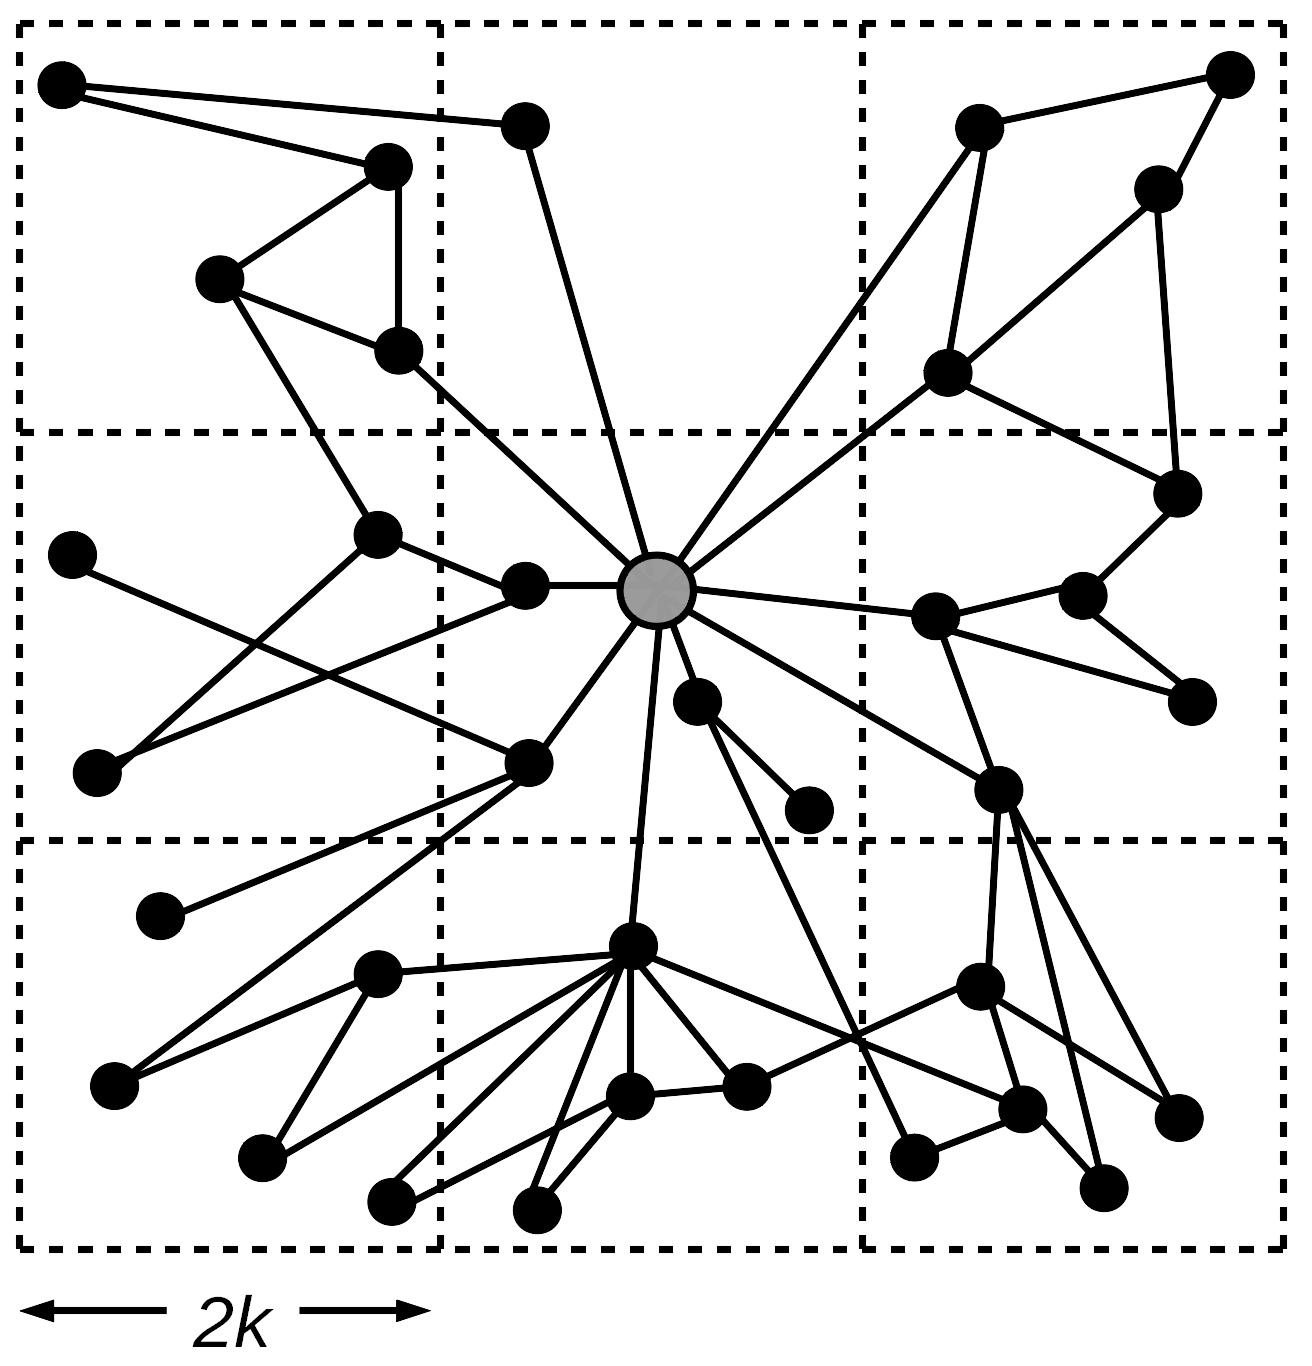
\includegraphics[width=0.95\textwidth]{graphTraversing_orig.png}
\caption[Graph mit $|V|=36$ und $|Gitterboxen|=9$]{Graph mit $|V|=36$ und $|Gitterboxen|=9$, eigene Darstellung}
\label{graphTraversing_orig}
\end{subfigure}
\hfill
\begin{subfigure}[t]{0.45\textwidth}
\centering
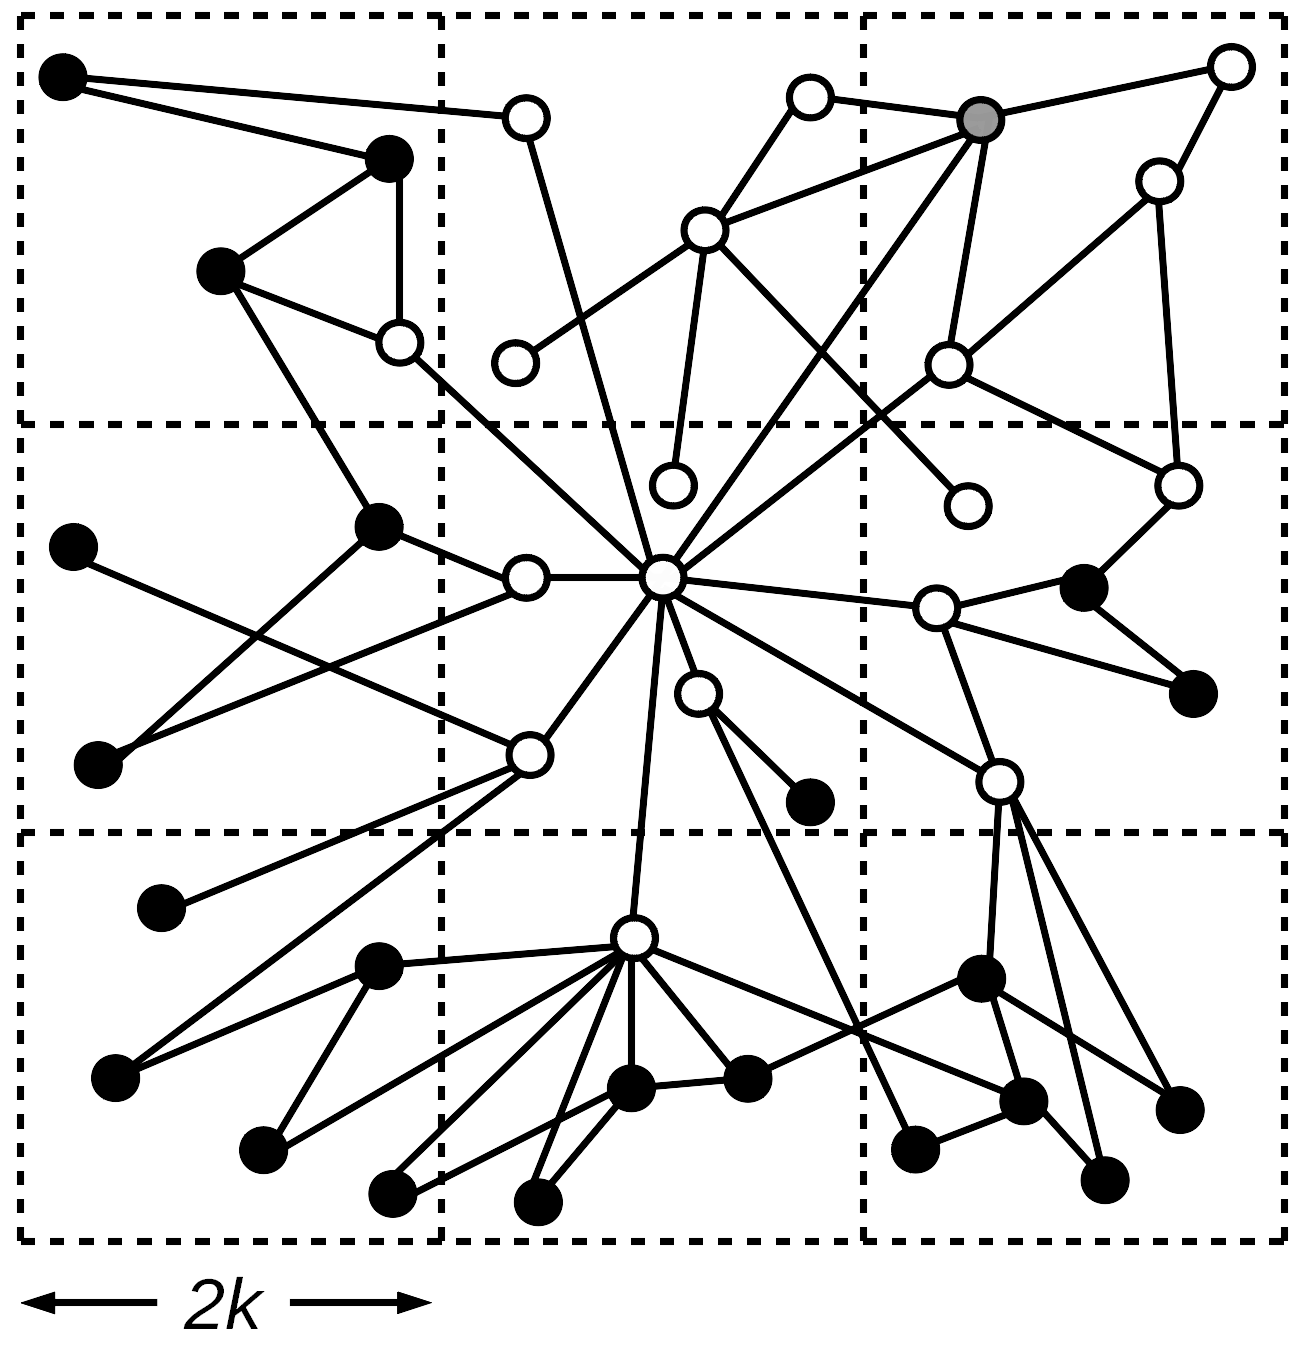
\includegraphics[width=0.95\textwidth]{graphTraversing_combined.png}
\caption["`Ausklappen"' eines neuen Knotens]{"`Ausklappen"' eines neuen Knotens, eigene Darstellung}
\label{graphTraversing_combined}
\end{subfigure}

\vspace{0.5cm}
\begin{subfigure}[t]{0.7\textwidth}
\centering
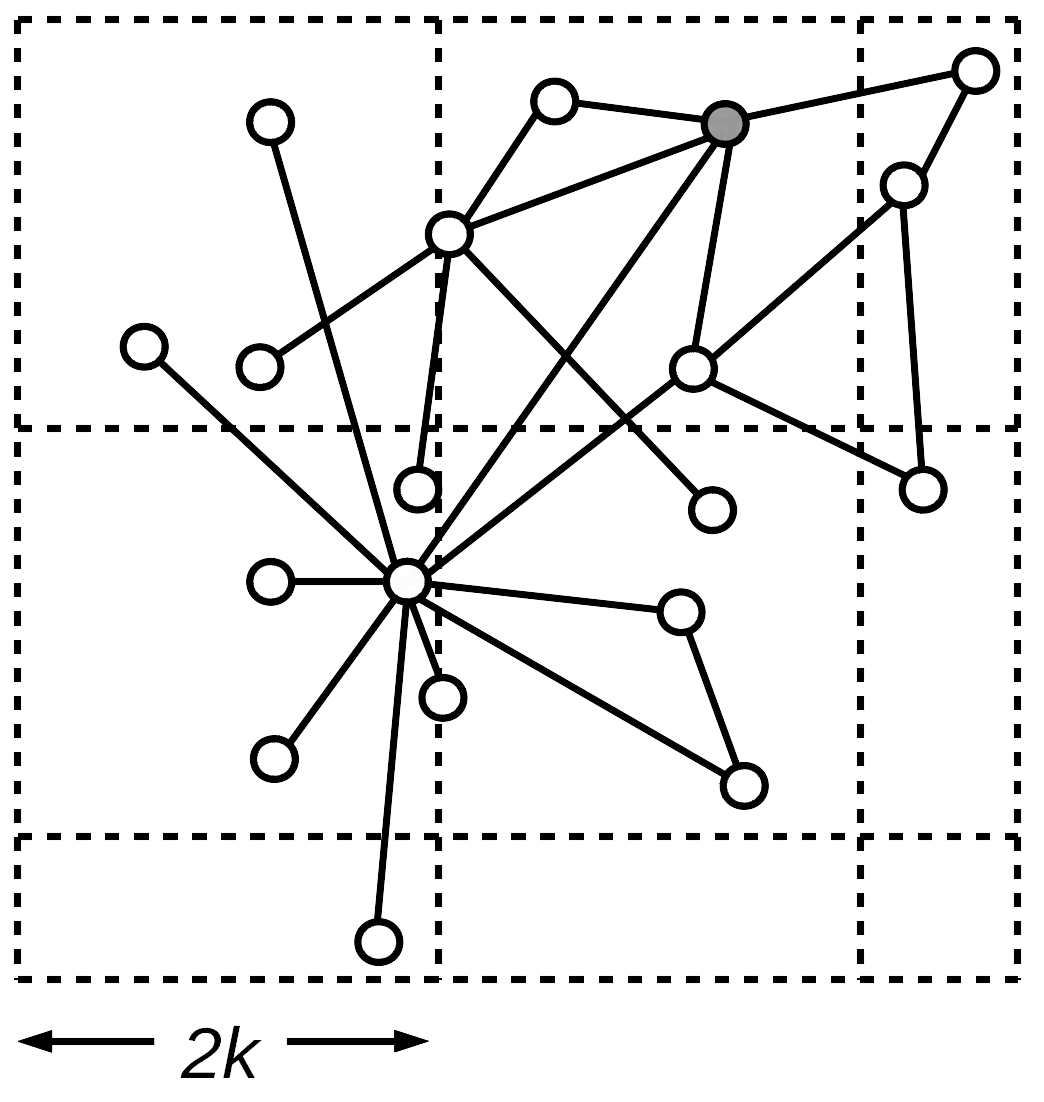
\includegraphics[width=0.95\textwidth]{graphTraversing_new.png}
\caption[Graph, der durch Löschen unerreichbarer Knoten entsteht]{Graph, der durch Löschen unerreichbarer Knoten entsteht, eigene Darstellung}
\label{graphTraversing_new}
\end{subfigure}
\caption{Ausklappen eines neuen Knotens}
\end{figure}

\subsubsection{Steuerung und Manipulation des Graphen}
Das vorgestellte Konzept zur Visualisierung der Wikipedia als Wissensgraph beruht darauf, dem Nutzer eine natürliche Interaktion mit diesem in einem virtuellen Raum zu ermöglichen. Der Nutzer soll mit dem Graphen interagieren können, als sei der Graph nicht nur eine dreidimensionale Zeichnung, sondern ein Objekt im Raum. Damit dieser Eindruck entsteht, wird dem Nutzer die Möglichkeit gegeben, nicht nur den Graphen von allen Seiten aus betrachten zu können, sondern diesen auch drehen zu können und sich in dem Raum, in dem der Graph dargestellt wird, bewegen zu können.\\

Der Nutzer interagiert mithilfe zweier Controller mit der Welt, einer in der linken und einer in der rechten Hand. Diese beiden Controller werden auch in der virtuellen Umgebung dargestellt, damit der Nutzer die Position seiner Hände im Blick hat und nicht bei der Interaktion mit dem Graphen gezwungen ist, die Immersion in der virtuellen Welt zu unterbrechen. Um den Graphen zu drehen, platziert der Nutzer seinen Controller an einem Punkt in der Welt und hält diesen durch Drücken eines Knopfes auf dem Controller fest. Anschließend kann er seinen Controller in eine beliebige Richtung bewegen, wodurch der Graph entlang dieser Richtung gedreht wird. Der Nutzer dreht also den Graphen, als würde er ihn an einer Stelle festhalten und in eine beliebige Richtung ziehen. Der Mittelpunkt der Rotation ist dabei immer der Mittelpunkt des Raums, in dem der Graph dargestellt wird.\\

Damit der Nutzer sich frei in der Welt bewegen kann, positioniert er seinen Controller an einer beliebigen Stelle im Raum. Danach hält er einen Knopf am Controller fest und zieht diesen in eine beliebige Richtung. Der gezeichnete Graph, falls einer vorhanden ist, wird nun entlang dieser Richtung verschoben. Dies ermöglicht dem Nutzer, weit entfernte Knoten zu erreichen und sich in allen drei Dimensionen durch den Raum zu bewegen.\\

Zusätzlich zu diesen grundlegen Arten, sich im Raum zu orientieren und sich fortzubewegen, wird dem Nutzer ermöglicht, einen neuen Knoten im Graph auszuwählen. Daraufhin bekommt er die Möglichkeit, sich den Artikel, der von dem Knoten repräsentiert wird, anzuzeigen. Auch bekommt er die Option, den neu ausgewählten Knoten zu fokussieren und als neuen Startknoten auszuwählen. Wählt er diese Option aus, wird der Graph daraufhin neu gezeichnet.\\

Als letztes wird zur Manipulation des Graphen noch ein Parametermenü angezeigt, welches der Nutzer anpassen kann. Mit diesem kann er die Anzahl der dargestellten Knoten und die Anzahl an erlaubten Sprüngen vom Startknoten aus festlegen. Die Änderungen an diesen Parameter werden wirksam, sobald der Nutzer den Graph erneut zeichnen lässt.\\

\subsubsection{Steuerung und Manipulation einzelner Artikel}
Ist ein bestimmter Knoten im Graphen ausgewählt, kann sich der Nutzer den Inhalt dessen anzeigen lassen. So ein Knoten besteht, wie bereits in Kapitel 3.1.2 erwähnt, aus mehreren Teilelementen. Diese Elemente werden nicht zusammen auf einer Seite dargestellt, wie es beim Abruf eines Wikipedia Artikels über einen Browser am Computer üblich wäre. Stattdessen wird jedes Element dem Nutzer einzeln manipulierbar zu Verfügung gestellt. Dadurch bekommt der Nutzer die Möglichkeit, sich viele Informationen gleichzeitig anzeigen zu lassen.\\

Ähnlich wie mit der Fortbewegung im Raum kann mit einem Controller auf eines der Elemente gezeigt werden und dieses damit ausgewählt werden. So kann der Nutzer Audio- und Videodateien auswählen und abspielen. Außerdem kann er die einzelnen angezeigten Elemente festhalten und verschieben. Dafür hält er eines der Elemente mit einem Knopfdruck fest und zieht es in eine beliebe Richtung. Abb.~\ref{articleInVR} zeigt, wie die Bewegung aus der Realität in der virtuellen Umgebung mit dem Artikelelement umgesetzt wird. Das Element folgt der Bewegung, die mit dem Controller ausgeführt wird und kann so beliebig im Raum verschoben werden. Der Nutzer kann so mit den Informationen umgehen und sie so arrangieren, als hätte er sie auf Haftnotizen vor sich.\\

\begin{figure}[h!]
\centering
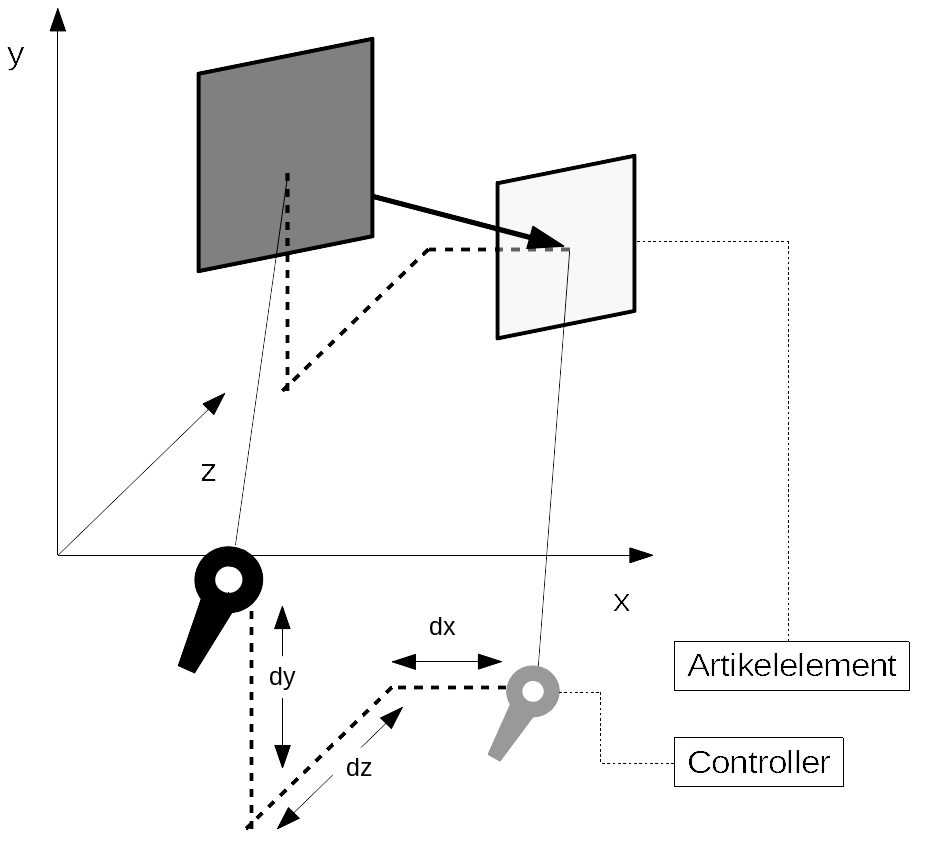
\includegraphics[width=0.95\textwidth]{interactionVR.png}
\caption[Darstellung einzelner Artikelinhalte in VR]{Darstellung einzelner Artikelinhalte in VR, eigene Darstellung}
\label{articleInVR}
\end{figure}
Um sicherzustellen, dass der Nutzer einzelne Elemente nicht versehentlich sehr weit wegschiebt und nicht mehr wiederfinden kann, muss es eine Funktion geben, um die Positionen der Elemente des Artikels zurücksetzen zu können. Dies kann als weiterer Knopfdruck oder auch als auswählbare Funktion im Interface eingebaut werden. Zuletzt muss dem Nutzer eine Funktion zu Verfügung gestellt werden, die es ermöglicht, den Artikelinhalt nach Belieben ein- oder auszublenden, damit die Navigation im Graph nicht zu unübersichtlich werden kann.\\

\subsubsection{Theoretischer Aufbau einer Anwendung zur Visualisierung der Wikipedia in VR}
Ein Konzept zur Visualisierung der Wikipedia in einer virtuellen Umgebung kann nun unter Beachtung der bisher aufgeführten Funktionen und Voraussetzungen formuliert werden.
Der grobe Aufbau der Anwendung kann in drei Komponenten aufgeteilt werden:
\begin{itemize}
\item Logik, übernimmt Interaktion mit dem Internet und Verarbeitung von Anfragen aus dem User Interface
\item Visualisierer, übernimmt Berechnung von Knotenpositionen in VR
\item Graph, übernimmt interne Darstellung und Struktur ausgelesener Artikel
\end{itemize}

Die Logik-Komponente widerum lässt sich in zwei grobe Unterkomponenten teilen. Die erste übernimmt die Interaktion mit dem Internet und das korrekte Auslesen und Weiterreichen von Daten. Sie ist dafür zuständig, dass aus dem Quellcode eines beliebigen Artikels Teilelemente herausgelesen werden. Zudem erfolgt hier die Breitensuche nach Links von einem Startartikel zu weiteren Artikeln. Alle Informationen, die aus dem Internet geholt werden müssen, werden in dieser Komponente verarbeitet. Die zweite Komponente verarbeitet alle Aktionen des Nutzers und leitet diese, wenn nötig, an die anderen Komponenten weiter. Darunter fallen Anpassungen der verfügbaren Parameter durch das Interface, Rotieren und verschieben des Graphen oder der Artikelelemente und Verändern der Position des Benutzers.\\

Der Visualisierer implementiert den in Kapitel 3.2.1 und 3.2.2 vorgestellten Algorithmus.\\

Die Graph-Komponente umfasst das Speichern von Knoten, Kanten und Artikelinformationen. Die Knoten und Kanten werden intern als Listen gespeichert, um ohne weiteres vom Visualisierer verarbeitet werden zu können. Kanten bestehen aus drei Informationen: dem Anfangsknoten, dem Endknoten und Auskunft über Gegenläufigkeit der Kante. Knoten speichern ihre Position, ihren Verschiebungsvektor für den Visualisierer, ihren Titel, ihre Anzahl an Aufrufen und inhaltliche Informationen. Die inhaltlichen Informationen wiederum repräsentieren die Teilelemente des Artikels, wie sie in 3.1.2 vorgestellt wurden.\\

Der Aufbau ist zur Verdeutlichung in Abb.~\ref{anwendungAufbau} grob bildlich dargestellt.\\

\begin{figure}
\centering
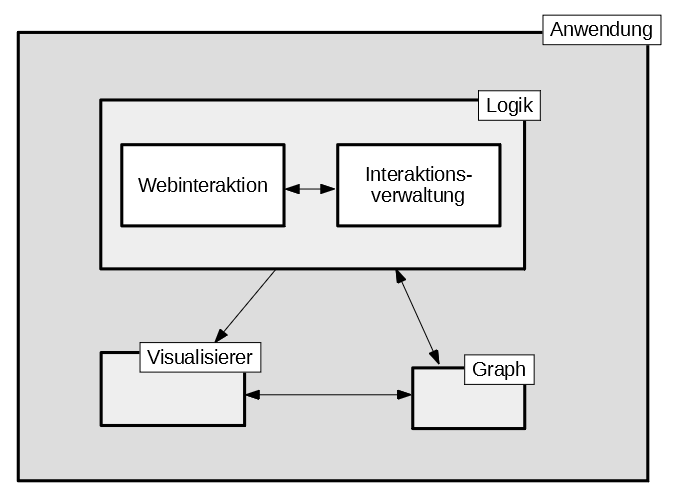
\includegraphics[width=0.8\textwidth]{Anwendung_Struktur.png}
\caption[Grober Aufbau einer möglichen Anwendung zur Visualisierung eines Graphen in VR]{Grober Aufbau einer möglichen Anwendung zur Visualisierung eines Graphen in VR, eigene Darstellung}
\label{anwendungAufbau}
\end{figure}

Wenn der Nutzer die Anwendung startet, bekommt er die Möglichkeit nach einem Artikel in der Wikipedia zu suchen oder einen zufälligen Artikel angezeigt zu bekommen. Ist der Startartikel bestimmt, werden von der Logik-Komponente mithilfe einer Breitensuche verlinkte Artikel als Nachbarknoten aufgenommen und in Knoten- und Kantenliste eingetragen. Die Breitensuche wird auf eine Tiefe begrenzt, die dem Nutzer als veränderbarer Parameter angezeigt wird. Dieser Parameter entspricht der Sprungzahl, die in Kapitel 3.1.3 erläutert wird. Ein zweiter veränderbarer Parameter, die Anzahl an maximal darzustellenden Knoten, bestimmt im nächsten Schritt, ob alle gefundenen Knoten an den Visualisierer weitergegeben werden. Ist die Anzahl an gespeicherten Knoten zu groß, werden die Knoten mit den niedrigsten Aufrufzahlen entfernt. Anschließend werden vom Visualisierer die Positionen aller relevanten Knoten berechnet und diese zusammen mit ihren Kanten in der virtuellen Umgebung dargestellt.\\

Der Nutzer kann nun frei mit dem Graphen interagieren. Er kann einen Knoten auswählen und näher betrachten, den Graph drehen und sich in diesem bewegen. Wird ein Knoten ausgewählt, kann der Nutzer sich dessen Inhalt anzeigen lassen oder den Graphen neu berechnen lassen (sofern nicht der ursprüngliche Startknoten ausgewählt wurde).\\

\newpage
\section{Implementierung}
\subsection{Importieren von Knoten, Kanten und Artikelinhalten aus dem Internet}
Es gibt mehrere Möglichkeiten, Informationen über einen Artikel in der Wikipedia über das Internet zu beziehen. Eine besonders simple ist es, den Quellcode der Seite anzufordern. In Unity sendet man dafür beispielsweise eine GET-Anfrage mit dem URL "`\url{https://de.wikipedia.org/wiki/Pink_Floyd}"' um den Quellcode des Artikels "`Pink Floyd"' zu erhalten. Problem hierbei ist es, relevante Informationen aus dem Text zu lesen. Da der Text in HTML vorliegt, sind viele für das korrekte Darstellen eines Artikels im Browser wichtige Informationen für die vorgestellte Anwendung unnötig.\\

Eine andere Möglichkeit bietet MediaWiki als "`MediaWiki Internetservice API"' an. Diese API kann verwendet werden, um gezielte Anfragen an eine MediaWiki Installation, so wie der Wikipedia, zu senden. Die Antwort vom Server kommt im JSON-Format. Um eine Anfrage an die deutsche Wikipedia zu senden verwendet man den URL "`\url{https://de.wikipedia.org/w/api.php?}"'. Als nächstes kann man dem URL mehrere Parameter hinzufügen.\\

In Unity ist es nicht ohne weiteres möglich, dynamische JSON-Antworten zu verarbeiten. Die Umgebung stellt eine Funktion zu Verfügung, die es ermöglicht ein JSON einer bestimmten Form auf eine Klasse mit dazu passenden Variablen abzubilden, d.h. sind alle Werte, die im JSON vorkommen, im Voraus bekannt, kann eine passende Klasse erstellt werden. In der Implementation ist meist nicht im Voraus klar, welche Form die Antwort des Servers haben wird oder wie viele Elemente darin enthalten sind. Stattdessen werden in der Implementation die Methoden der string-Klasse verwendet, um primitive Umformungen anzuwenden. Im folgenden Code aus der Implementation ist die Antwort des Servers im JSON-Format in der Variable "`content"' gespeichert. Hier wird mithilfe der Methode "`IndexOf(string val)"' die Position gefunden, an der die Variable "`title"' steht. Danach wird die Position des ersten Zeichens und die Position des ersten Zeichens nach dem Titel ermittelt. Der gesuchte Titel befindet sich nun zwischen den beiden genannten Positionen.
\begin{lstlisting}
int pos1 = content.IndexOf("title");
pos1 = pos1 + 8;
int pos2 = content.LastIndexOf("\"");
content = content.Remove(pos2, content.Length-pos2);
content = content.Remove(0, pos1);
\end{lstlisting}
Im vorgestellten Konzept starten wir immer mit einem ausgewählten Artikel. Um eine Liste aller Links von einem Artikel aus auf andere zu erhalten, verwendet die Implementation die Parameter und zugehörigen Werte "`action=query"' und "`prop=links"', wobei der erste Parameter verwendet wird, um Daten vom Server zu beziehen, der zweite, um speziell Links einer Seite zu erhalten. Als nächstes verwendet die Implementation zusätzlich den Parameter "`plnamespace=0"', welcher dem Server mitteilt, dass nur Links zu anderen Wikipedia-Artikeln angefragt werden. Die Wikipedia besteht aus mehreren Gruppen von unterschiedlichen Seiten, genannt Namensräume. Der Namensraum 0 umfasst hierbei alle enzyklopädischen Artikel der Wikipedia und wird auch Artikelnamensraum genannt. Andere Namensräume sind beispielsweise 1, für Diskussionsseiten, oder 2, für Benutzerseiten. In der Implementation wird zusätzlich der Parameter "`format=json"' verwendet, um eine Antwort im JSON-Format zu erhalten.\\

Ein weiterer Parameter, der verwendet wird, ist "`pllimit=max"', welcher dem Server mitteilt, dass die maximale Anzahl an verfügbaren Ergebnissen angefragt wird. Normale Nutzer können maximal 500 Ergebnisse anfragen. Gibt es mehr als 500 Ergebnisse, steht in der Antwort vom Server ein Bereich mit Namen "`continue"', in dem zwei Werte enthalten sind. Ein Wert trägt den Namen "`plcontinue"' und kann dafür verwendet werden, eine neue Anfrage an den Server zu schicken. Der Wert des Parameters "`plcontinue"' im verwendeten URL gibt dem Server die Stelle an, ab der weitere Ergebnisse geladen werden sollen. Der letzte verwendete Parameter ist "`titles"'. Der Wert dieses Parameters ist der Titel, für den Links angefordert werden sollen. Eine Anfrage, um beispielsweise alle Links auf der Seite "`Pink Floyd"' herauszufinden, lautet dann "`\url{https://de.wikipedia.org/w/api.php?action=query&format=json&prop=links&plnamespace=0&pllimit=max&titles=Pink_Floyd}"'.\\

Auf ähnliche Art aber mit anderen Parametern, bzw. Werte für diese Parameter, können auch weitere Informationen bezogen werden. Für eine Liste zufälliger Artikel beispielsweise kann der Parameter "`list=random"' verwendet werden. Mit "`rnlimit=1"' zusätzlich wird die Liste auf ein Element beschränkt. Diese Anfrage wird in der Implementation verwendet, um einen zufälligen Artikel der deutschen Wikipedia zu erhalten.\\

Die Paragraphen eines Artikels können auch abgefragt werden. Hierzu verwendet die Implementation den Parameter "`prop=extracts"'. Dieser Parameter gehört zu einer Erweiterung der MediaWiki Internetservice API, welcher es ermöglicht Paragraphen im Textformat und ohne HTML Formatierung zu erhalten.\\

Wie bereits in Kapitel 3.1.3 erwähnt, gibt es Parameter, die das Aussehen und das Ausmaß des zu zeichnenden Graphen beeinflussen. Mithilfe dieser Parameter kann eine Methode formuliert werden, die, ausgehend von einem gegebenen Artikel, einen Graphen erstellt. Der folgende (verkürzte) Code gibt den Aufbau und die Funktionsweise dieser Methode wieder. Die Variable "`nodesToCheck"' speichert hierbei eine Liste von Knoten, die erkundet werden sollen. Vor Beginn der ersten Schleife steht in dieser Liste nur der gewählte Startknoten. Die Variable "`hops"' speichert die Anzahl an erlaubten Sprüngen.
\begin{lstlisting}
for (int i = 0; i < hops; i++)
{
	int currentNodesToCheck = nodesToCheck.Count;
	for (int j = 0; j < currentNodesToCheck; j++)
	{
		yield return StartCoroutine(
          communicator.requestNeighbors(
          nodesToCheck[j].getName()));
		List<string> tempNeighbors =
          communicator.getNeighbors();
		for (int z = 0; z < tempNeighbors.Count; z++)
		{
			nextNode = ...
			// Fuege nextNode und Kante in den Graphen ein,
			// falls diese noch nicht im Graphen vorkommen
			... 
			nodesToCheck.Add(nextNode);
		}
	}
	nodesToCheck.RemoveRange(0, currentNodesToCheck);
	// Dieser Schritt entfernt die ersten
    // |currentNodesToCheck| Knoten aus der Liste,
    // auf der wir arbeiten.
}
\end{lstlisting}
In die Liste "`nodesToCheck"' werden alle Nachbarn eines betrachteten Knoten eingefügt. Wurde die Nachbarschaft eine Knotens abgearbeitet, wird sie aus der Liste entfernt und der Algorithmus macht mit dem nächsten Knoten weiter.\\

Ein Problem, welches beim Anfragen und Erhalten von Informationen über die MediaWiki Internetservice API auftritt, ist die Dauer der Anfragen. Beim Testen des obigen Codes für einen beliebigen Artikel und eine Sprungzahl von 2 braucht die Implementation sehr lange, um alle Knoten zu erkunden. Mit dem Artikel "`Roger Waters"' und einer Sprungzahl von 2 beispielsweise, also ein Graph mit dem genannten Artikel, dessen Nachbarn und die Nachbarn dieser Nachbarn, dauerte das Ausführen der Methode 294,312 Sekunden oder etwa 4,9 Minuten. Die Anzahl an Knoten, die der Graph umfasst, war 25311. Eine einzige Anfrage an die API, alle Nachbarn eines gegebenen Artikels zu erhalten, dauerte bei 10 gemessenen Werten im Schnitt 0,2751 Sekunden.\\

\newpage
\subsection{Modellierung eines User Interfaces}
Die direkte Interaktion mit dem gezeichneten Graph in VR erfolgt durch Verschieben und Rotieren des Graphen. Dazu werden die Trigger-Knöpfe auf der Hinterseite der HTC Vive Controller verwendet. Bei Festhalten des Trigger-Knopfes am linken Controller, lässt sich durch gleichzeitiges Bewegen des Controllers der Graph verschieben. Bei Festhalten des Triggers am rechten Controller lässt sich der Graph rotieren. Die Umsetzung dieser Funktionalität erfolgt in der Implementierung allerdings nicht über ein geteiltes Skript. Stattdessen verwenden der linke und der rechte Controller jeweils ein angepasstes Skript. Die HMD- und Controllerfunktionalität wird von einem Paket namens "`SteamVR"' bereitgestellt, welches als Plug-in für Unity zu Verfügung steht. Das Plug-in stellt eine angepasste Kamera bereit, die die beiden Controller verwaltet. Diese Controller werden von einem Skript beobachtet. Ein weiteres Skript sendet an alle weiteren Komponenten des Controllers Nachrichten, sobald eine Eingabe am Controller festgestellt wird, also beispielsweise das Berühren des Touchpads oder Drücken eines Knopfes.\\

Der untenstehende Code ist ein Ausschnitt des Skriptes, welches dem linken Controller zugeordnet ist. Der Variable "`controller"' wird in der Methode "`OnEnable()"' das Skript zugewiesen, welches die Nachrichten bei Eingabe am Controller verschickt. Der Variable "`GraphContainer"' wird der gezeichnete Graph zugewiesen. Die Methode "`Update()"' wird von Unity jedes Frame aufgerufen und prüft hier, ob der Trigger des linken Controllers gerade gedrückt wird. Falls ja, wird der Vektor zwischen der letzten gemessenen Position des Controllers und der aktuellen Position des Controllers berechnet und auf das Objekt angewandt, welches den Graphen repräsentiert. In der Methode "`OnEnable()"' wird hier festgelegt, welche weitere Methode der Klasse beim Drücken eines bestimmten Knopfes aufgerufen werden sollen, siehe Zeile 25 und Zeile 26.
\begin{lstlisting}
private SteamVR_TrackedController controller;
public GameObject GraphContainer;
private Vector3 lastPos;
private bool isTriggerDown = false;

private void Start()
{
	lastPos = this.transform.position;
}

private void Update()
{
	if (isTriggerDown)
    {
    	GraphContainer.transform.position +=
          this.transform.position - lastPos;
    }
	lastPos = this.transform.position;
}

private void OnEnable()
{
	controller = GetComponent<SteamVR_TrackedController>();
	...
	controller.TriggerClicked += activateTrigger;
	controller.TriggerUnclicked += deactivateTrigger;
	...
}
\end{lstlisting}
Das konzipierte User Interface ist darauf angepasst, innerhalb einer VR-Umgebung zu existieren. Das heißt, das Menü existiert im dreidimensionalen Raum, nicht als Overlay im sogenannten "`Screen Space"'. Der Screen Space beschreibt die Fläche, die den Screen umfasst. Beim Arbeiten mit einem HMD lässt sich auch eine Art Overlay konzipieren, auf dem der Nutzer gewissen Werte im Blick hat. Dieses ist allerdings, im Gegensatz zur Anwendung auf einem typischen Computerbildschirm, nicht unbedingt für interaktive Menüs geeignet. Der Nutzer verwendet zwei Controller im dreidimensionalen Raum, weshalb das Menü auch als Teil des Raumes umgesetzt wird.\\

Das Auswählen gewisser Menüpunkte erfolgt über sogenanntes "`Raycasting"'. In der Implementierung wird hierbei von dem Controller aus in die Richtung, in die dieser zeigt, eine Linie gezeichnet. Trifft diese Linie auf einen Menüpunkt, kann dieser ausgewählt und manipuliert werden.\\

\newpage
\subsection{Umsetzung des Visualisierungsalgorithmus}
Wie bereits in Kapitel 2.4 erwähnt und in Kapitel 3.2.1 näher erläutert, gliedert sich der Algorithmus in drei Hauptabschnitte. In der Implementation werden zuerst zwischen allen möglichen Knoten abstoßende Kräfte berechnet. Da die berechneten Verschiebungsvektoren erst im dritten Hauptabschnitt angewandt werden, macht es hier keinen Unterschied, ob zuerst abstoßende oder anziehende Kräfte berechnet werden. Der folgende Code berechnet alle abstoßenden Kräfte und daraus resultierende Verschiebungsvektoren zwischen allen Knoten des Graphen.
\begin{lstlisting}
foreach (Graph.Node currentNode in nodes)
{
	currentNode.setDisplacement(0.0f, 0.0f, 0.0f);
    
	foreach (Graph.Node node in nodes)
	{
		if (currentNode != node)
		{
			// Differenzvektor := v.pos - u.pos
			float differenceX =
              currentNode.getX() - node.getX();
			float differenceY =
              currentNode.getY() - node.getY();
			float differenceZ =
              currentNode.getZ() - node.getZ();

			float differenceLength = Mathf.Sqrt(
              differenceX * differenceX +
              differenceY * differenceY +
              differenceZ * differenceZ);

			// v.disp := v.disp + (Dif.vektor / |Dif.vektor|)
			// * repulsiveForce(|Dif.vektor|)
			float repulsiveForce =
              getRepulsiveForce(differenceLength);
                
			currentNode.addDisplacement(
              (differenceX / differenceLength) *
              repulsiveForce,
              (differenceY / differenceLength) *
              repulsiveForce,
              (differenceZ / differenceLength) *
              repulsiveForce);
		}
	}
}
\end{lstlisting}
Die Variable "`nodes"' beinhaltet eine Liste aller Knoten des Graphen. Die erste Schleife geht hier alle Knoten des Graphen durch und setzt den zugehörigen Verschiebungsvektor als erstes auf $(0, 0, 0)^T$. In der zweiten Schleife werden alle anderen Knoten des Graphen durchgegangen. Die Zeilen 10 bis 15 berechnen die Werte des Vektors zwischen den beiden betrachteten Knotenpunkten. Mit diesen Werten wird als nächstes die Länge des Vektors berechnet. Diese wird schließlich in Zeile 24 und Zeile 25 verwendet, um die abstoßende Kraft auf den aktuellen Knoten, "`currentNode"', von dem betrachteten Knoten aus, "`node"', zu berechnen. In Zeile 27 bis 33 wird mithilfe der Werte des Differenzvektors, dessen Länge und der eben berechneten repulsiven Kraft der Verschiebungsvektor zu "`currentNode"' berechnet. Dieser Abschnitt des implementierten Algorithmus hat eine Laufzeit von $O(|Kanten|^2)$ und ist somit der rechenaufwendigste Teil des Algorithmus.\\

Im zweiten Hauptabschnitt des Algorithmus werden die anziehenden Kräfte zwischen allen verbundenen Knoten berechnet. Dafür wird die Liste an Kanten, hier "`edges"', durchgegangen.
\begin{lstlisting}
foreach (Graph.Edge edge in edges)
{
	//Differenzvektor := e.v.pos - e.u.pos
	float differenceX =
      edge.getFrom().getX() - edge.getTo().getX();
	float differenceY =
      edge.getFrom().getY() - edge.getTo().getY();
	float differenceZ =
      edge.getFrom().getZ() - edge.getTo().getZ();

	float differenceLength = Mathf.Sqrt(
      differenceX * differenceX +
      differenceY * differenceY +
      differenceZ * differenceZ);
	float attractiveForce =
      getAttractiveForce(differenceLength);

	//e.v.disp := e.v.disp - (Dif.vektor / |Dif.vektor|) *
    // attractiveForce(|Dif.vektor|)
	edge.getFrom().setDisplacement(
    	edge.getFrom().getDisplacementX() -
        (differenceX / differenceLength) * attractiveForce, 
        edge.getFrom().getDisplacementY() -
        (differenceY / differenceLength) * attractiveForce, 
        edge.getFrom().getDisplacementZ() -
        (differenceZ / differenceLength) * attractiveForce);

	//e.u.disp := e.u.disp + (Dif.vektor / |Dif.vektor|) *
    // attractiveForce(|Dif.vektor|)
	edge.getTo().setDisplacement(
      edge.getTo().getDisplacementX() -
      (differenceX / differenceLength) * attractiveForce,
      edge.getTo().getDisplacementY() -
      (differenceY / differenceLength) * attractiveForce,
      edge.getTo().getDisplacementZ() -
      (differenceZ / differenceLength) * attractiveForce);
}
\end{lstlisting}
Auch dieser Abschnitt beginnt damit, die Werte des Differenzvektors zwischen zwei Knoten auszurechnen, hier nämlich zwischen den beiden Knoten, die die Kante "`edge"' verbindet. Wie bei den anziehenden Kräften wird wieder die Länge dieses Vektors berechnet und mithilfe dessen die anziehende Kraft zwischen den beiden Knoten berechnet. In Zeile 20 bis 26 wird auf den Verschiebungsvektor des ersten Knotens der Kante diese Kraft angewandt. Es wird hier der neu anzuwendende Verschiebungsvektor vom bereits bestehenden Verschiebungsvektor abgezogen und nicht, wie bei der Berechnung der abstoßenden Kräfte, addiert. Die gleiche Kraft wird nach demselben Prinzip in Zeile 30 bis 36 auch auf den zweiten Knoten der Kante angewandt.\\

\newpage
\subsection{Gegenüberstellung verschiedener Konfigurationen}
Durch die verschiedenen vorgestellten Parameter zur Visualisierung eine Graphen lassen sich auch verschiedene Messwerte für die Laufzeit der Implementierung vergleichen. In den folgenden Messergebnissen werden Laufzeiten für den Visualisierungsalgorithmus auf Basis von \citeA{fruchterman1991graph} für unterschiedliche Konfigurationen besprochen. Außerdem wird die Dauer des Algorithmus' besprochen, der die nötigen Informationen über Artikel und Links vom Server holt. Die vorgestellten Messwerte und Visualisierungen wurden alle mit dem gleichen Startknoten durchgeführt. Dieser ist der Wikipediaartikel "`Roger Waters"' mit 156 weiterführenden Links.\\

Die erste hier vorgestellte Messung bezieht sich auf den Graphen in Abb.~\ref{graph_1hop}. Besonders gut zu sehen ist hier die Sternstruktur, die man erhält, wenn man nur einen Sprung vom Startartikel auszulässt. Dieser Graph hat insgesamt $|V|=157$ Knoten und erlaubte Sprünge $|Hops|=1$, also den Startknoten und all dessen Nachbarn. Die Ausführung des Visualisierungsalgorithmus hat für diesen Graphen $T_{Visualisierung}=406 ms \approx 0,4 s$ gebraucht. Die Visualisierung erfolgte hier also in einer Geschwindigkeit, die für einen Menschen kaum wahrnehmbar ist. Der Algorithmus zum Aufbauen des Graphen mithilfe von Kommunikation mit dem Server hat im Verlgeich dazu $T_{Webinteraktion} = 407 ms \approx 0,4 s$ gebraucht, wobei dieser Wert je nach Konnektivität stark schwanken kann. In dieser Konfiguration wurde nur eine Anfrage an den Server gesendet. Der Algorithmus zu Visualisierung des Graphen und der Algorithmus zur Webinteraktion dauern in diesem Fall also nahezu gleichlang, die Visualisierung für den Nutzer wurde noch in unter einer Sekunde fertiggestellt.\\

Im Vergleich dazu wurde in Abb.~\ref{graph_2hop_250} die Sprungzahl auf $|Hops|=2$ erweitert. In Kapitel 4.1 wurde bereits erwähnt, dass mit dem gleichen Artikel und der gleichen Sprungzahl die Anwendung einfriert. Um dies zu Vermeiden, wurde für die hier abgebildete Visualisierung die maximale Anzahl an Knoten, angesprochen in Kapitel 3.1.3, auf 250 beschränkt. Die Visualisierung des Graphen hat dadurch etwas mehr als doppelt so lang gedauert, nämlich $T_{Visualisierung}=1000 ms = 1 s$. Das Anfragen von Informationen beim Server und die Verarbeitung derer hat hingegen $T_{Webinteraktion}=1907 ms \approx 1,9 s$ gebraucht. Diese Dauer kann bereits störend beim Verwenden der Anwendung wirken, wobei auch gut sichtbar ist, dass die Visualisierung unübersichtlicher ist, als in Abb.~\ref{graph_1hop}.\\

Da die Visualisierung in Abb.~\ref{graph_2hop_250} allerdings nur Nachbarn von einem einzigen Nachbarn des Startartikels anzeigt, wurde ein dritter und letzter Test durchgeführt. Hierfür wurde nicht die Anzahl an Knoten beschränkt, sondern die Anzahl an Nachbarn, die bei der Breitensuche vom Startknoten aus jeweils berücksichtigt werden. Der dargestellte Graph bricht nach 20 erkundeten Nachbarn ab und geht zum nächsten Knoten in der Liste über, wodurch jeder Knoten höchstens auf 20 weitere Knoten zeigt. Der vorgestellte Graph ist in Abb.~\ref{graph_2hop_neighborlimit} als Visualisierung der Anwendung dargestellt. Bei dieser Visualisierung lässt sich allerdings, im Gegensatz zu den Graphen aus Abb.~\ref{graph_1hop} und Abb.~\ref{graph_2hop_250}, eine stärkere Vernetzung im Zentrum des Graphen beobachten. Tatsächlich hat der in Abb.~\ref{graph_2hop_neighborlimit} dargestellte Graph eine Knotenzahl von $|V|=265$. Der Algorithmus zur Visualisierung hat hier $T_{Visualisierung}=1157 ms \approx 1,16 s$ gebraucht, was nicht viel länger ist, als die Visualisierung von Abb.~\ref{graph_2hop_250}. Die Dauer der Kommunikation mit Server und Verarbeitung von Informationen hat stattdessen mit $T_{Webinteraktion}=5906 ms \approx 5,9 s$ deutlich länger gebraucht.\\

Diese Ergebnisse zeigen sehr gut, dass das größte Problem bei der Reduzierung der Wartezeiten der Anwendung in der Kommunikation mit dem Internet liegen.
\begin{figure}
\centering
\begin{subfigure}[t]{0.45\textwidth}
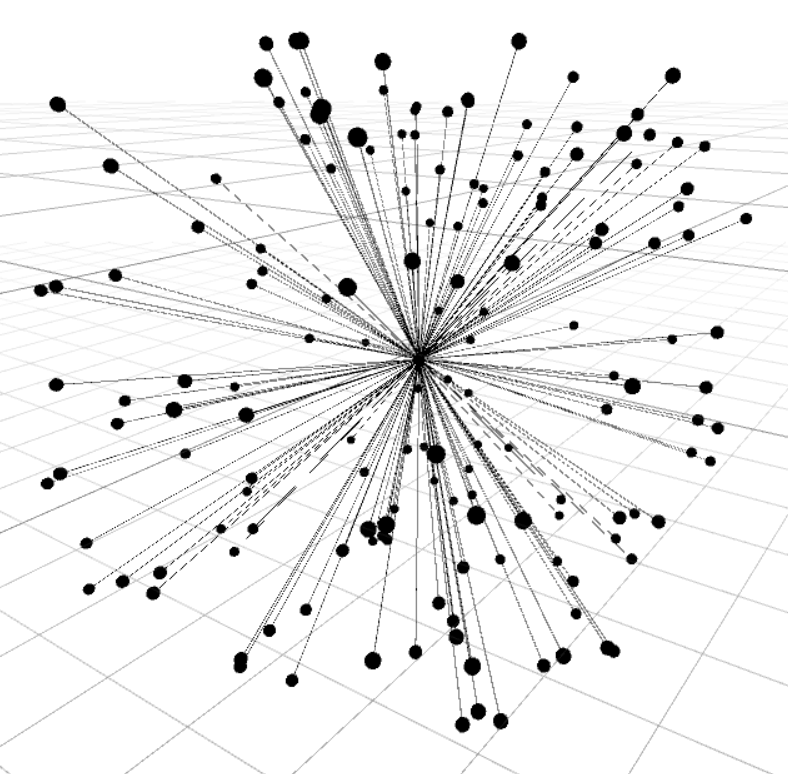
\includegraphics[width=0.9\textwidth]{Roger_Waters_1Hop_157Nodes_FR406_WEB407.png}
\caption[Visualisierter Graph mit $|V|=157$ und $|Spruenge|=1$]{Visualisierter Graph mit $|V|=157$ und $|Hops|=1$, eigene Darstellung}
\label{graph_1hop}
\end{subfigure}
\begin{subfigure}[t]{0.45\textwidth}
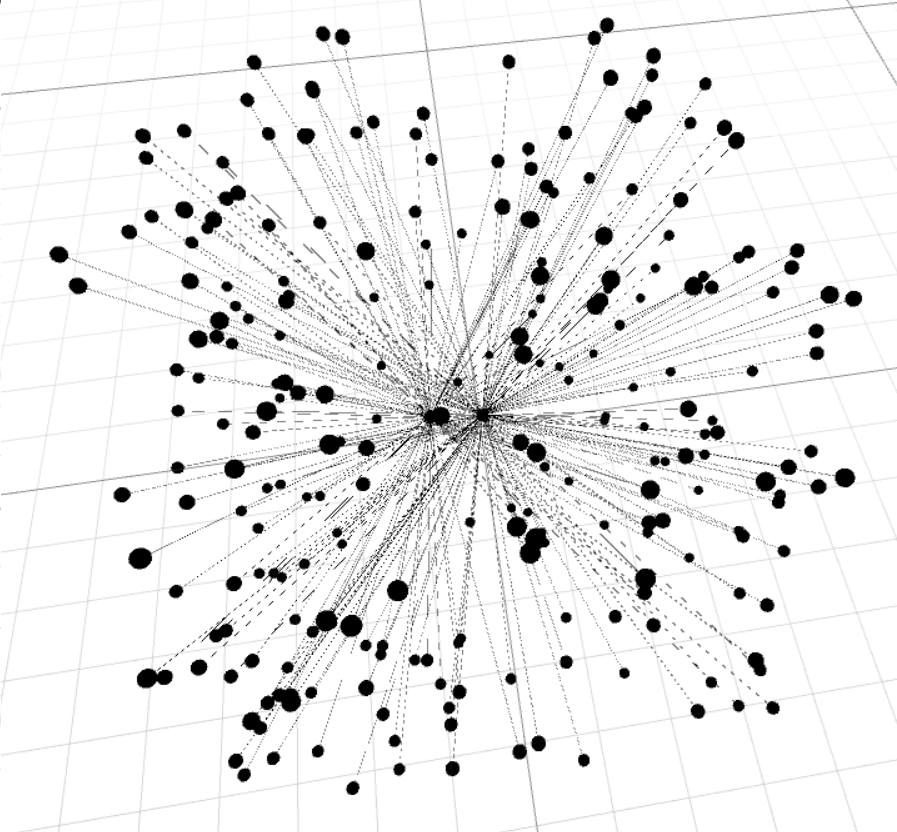
\includegraphics[width=0.9\textwidth]{Roger_Waters_2Hop_250Nodes_FR1000_WEB1907.png}
\caption[Visualisierter Graph mit $|V|=250$ und $|Hops|=2$]{Visualisierter Graph mit $|V|=250$ und $|Hops|=2$, eigene Darstellung}
\label{graph_2hop_250}
\vspace{0.5cm}
\end{subfigure}
\begin{subfigure}[t]{0.85\textwidth}
\centering
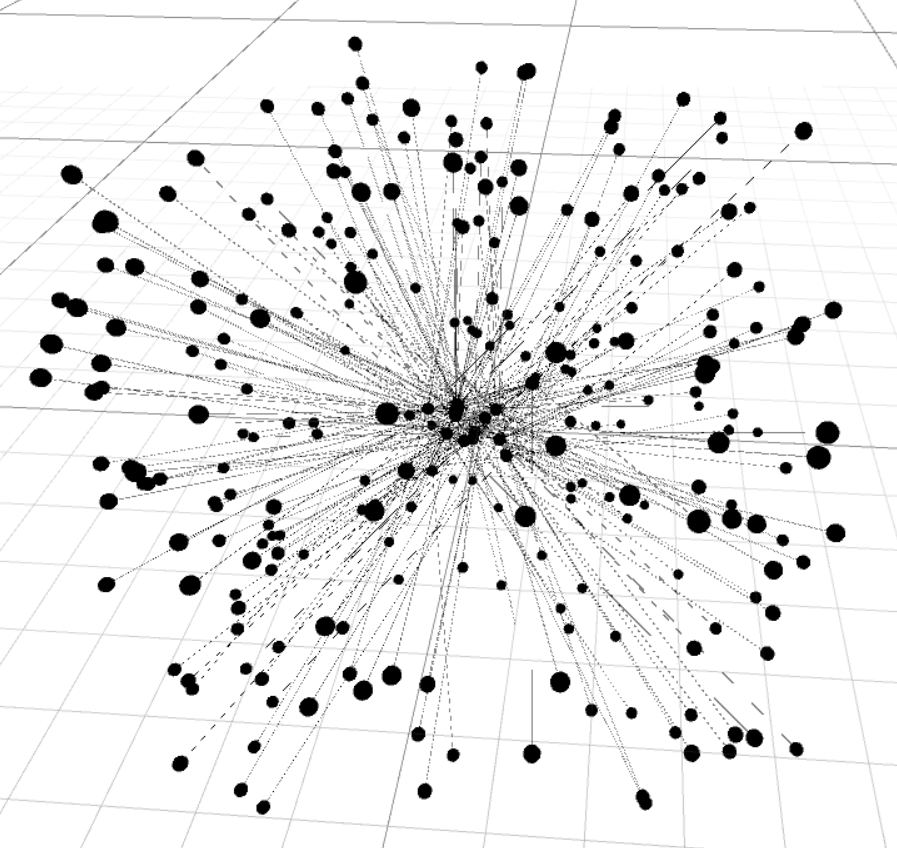
\includegraphics[width=0.9\textwidth]{Roger_Waters_2Hop_265Nodes_FR1157_WEB5906_neighborlimit20.png}
\caption[]{Visualisierter Graph mit $|V|=265$ und $|Hops|=2$, wobei nur die ersten 20 Links eines Artikels erkundet wurden, eigene Darstellung}
\label{graph_2hop_neighborlimit}
\end{subfigure}
\caption{Verschiedene Visualisierung eines Teilausschnitts der Wikipedia, ausgehend vom gleichen Startartikel, eigene Darstellung}
\end{figure}

\newpage
\subsection{Technische Daten des verwendeten Systems}
Das Projekt wurde in der Unity-Engine geschrieben, die einzelnen Skripte wurden in C\# geschrieben. Als VR-Lösung wurde die HTC Vive verwendet. Die Rotation und Position des HMD der HTC Vive wird mit zwei Sensoren getrackt. Zwei Controller, einer für die linke und einer für die rechte Hand, können vom Nutzer verwendet werden. Die Einbindung des VR-Systems in Unity erfolgte über das Unity-Plugin SteamVR. Die verwendete Unity-Version ist Unity 2017.3.0f3 und die Version des verwendeten SteamVR-Plugins ist 1.2.3. Die verwendete Entwicklungsumgebung zum Schreiben des Programmcodes in C\# ist Microsoft Visual Studio Enterprise 2017, Version 15.5.2.\\

Implementierung, Messungen und Tests wurden auf einem Rechner mit einem Intel Core i7-7700HQ Prozessor bei 2,80 GHz mit 4 echten Kernen durchgeführt. Die Grafikkarte des Geräts ist eine NVIDIA GeForce GTX 1070 mit 8 GB Speicher, der Arbeitsspeicher umfasst 16 GB. Das Betriebssystem des Rechners ist Windows 10 Education N.

\newpage
\section{Schluss}
In dieser Arbeit wurde ein Konzept zur Umsetzung einer Anwendung vorgestellt, welche einem Nutzer die Möglichkeit bietet, sich ein Wissensnetzwerk als Graph darstellen zu lassen, damit Verbindungen zwischen Artikeln und Informationen leichter ersichtlich sind. Hierfür wurden Grundlagen zur Graphentheorie und zu virtueller Realität vorgestellt.\\

Für die Formulierung des Konzeptes wurden verschiedene Teilabschnitte vorgestellt. Zuerst wurde die Wikipedia auf Struktur und Komplexität analysiert. Dabei wurde festgestellt, dass die Wikipedia aus sehr vielen Artikeln besteht, die bei der Darstellung im Graph begrenzt werden müssen, um den Benutzer nicht zu überfordern. Bei der Analyse wurde zudem festgestellt, dass Artikel nicht unbedingt einem einheitlichen Aufbau folgen, der zudem aus vielen verschiedenen Elementen bestehen kann. Mit diesen Erkenntnissen wurde ein Konzept zur Darstellung von Informationen vorgeschlagen, welcher das Darstellen aller verfügbaren Informationen in Etappen einteilt. Das beschriebene Konzept erlaubt es einem Nutzer, sich die Struktur der Wikipedia als Graph darstellen zu lassen, einzelne Artikel in ihren Bestandteilen zu betrachten und sich den Aufbau eines solchen Artikels ebenfalls als Graph darstellen zu lassen. Bei der Beschreibung dieses Konzepts wurde ersichtlich, dass Informationen, wie sie am Bildschirm anschaubar sind, im Raum platziert werden müssen, um dem Nutzer eine natürliche Interaktion mit der Anwendung zu ermöglichen.\\

Bei der Formulierung des Konzepts und Implementierung dessen mussten einige Einschränkungen gemacht werden. So kann beispielsweise im vorgestellten Konzept nur ein kleiner Teilausschnitt der Wikipedia visualisiert werden, der von einem gewählten Artikel aus aufgebaut wird. Außerdem wurde beim Testen der Implementation festgestellt, dass durch die Kommunikation mit dem Internet die einstellbaren Parameter zur Visualisierung eines Teilgraphen der Wikipedia nur zum Teil genutzt werden können. Hier wurde beispielsweise ein Parameter vorgestellt, der die maximale Entfernung zum Startartikel angibt, welcher aber bereits bei einer Entfernung von zwei Schritten die Anwendung durch die ausgiebige Internetkommunikation einfrieren lässt. Ein weiteres Problem lässt sich beim Umsetzen der Internetkommunikation beobachten. Hier wurde ersichtlich, dass die genutzte Umgebung zur Implementierung, Unity, dynamische Antworten eines Servers im JSON-Format nicht ohne weiteres verarbeiten kann. Dadurch wurde es nötig, stark angepasste Methoden zu implementieren, die sich nur darum kümmern, JSON-Antworten zu verarbeiten.\\

Trotz einiger Hindernisse und Probleme erfüllt das vorgestellte Konzept den Leitgedanken dieser Arbeit und kann als Grundgerüst zur Implementierung einer Visualisierungssoftware für Wissensnetzwerke in einer virtuellen Umgebung verwendet werden. Das Konzept erfüllt die Anforderungen, Artikel und deren Verbindungen in einem Wissensnetzwerk als Graph mit Knoten und Kanten zu visualisieren. Der Gedanke des Konstruktivismus, welcher in der Einleitung vorgestellt wurde, wird im vorgestellten Konzept zudem dadurch verfolgt, dass der Nutzer im virtuellen Raum den Graphen frei manipulieren oder traversieren kann und sich selber ein Bild zum Zusammenhang verschiedener Informationen machen kann.\\

Das vorgestellte Konzept soll allerdings prinzipiell nur als Grundgerüst betrachtet werden. Zusätzlich zu den vorgestellten Ideen lassen sich weitere Funktionen formulieren, die hier nicht behandelt wurden. Eine echte Filtrierung der Ergebnisse nach Kategorien wäre für einen Nutzer eventuell eine interessante Erweiterung. Die Implementierung leidet außerdem darunter, nur die Wikipedia als Wissensnetzwerk verwenden zu können. Hier könnte eine Erweiterung vorgestellt werden, die die verschiedenen Aspekte unterschiedlicher Netzwerke behandeln kann. Auch wird nur sehr oberflächlich auf die Teilelemente enzyklopädischer Einträge eingegangen, hier ließe sich das Konzept stark erweitern.\\

\newpage
\bibliographystyle{apacite}
\bibliography{bibliography}
\end{document}